\documentclass[aspectratio=169]{beamer}
\usetheme{SimpleDarkBlue}
\usecolortheme{default}
% \usefonttheme{serif}
\usepackage{helvet}
\usepackage[dvipsnames]{xcolor}
\usepackage{tabularx}
\usepackage{booktabs}
\usepackage[utf8]{inputenc}
\usepackage{longtable}
\usepackage{siunitx}
\usepackage{array, multirow, tabularx,tabu}

\usepackage[T1]{fontenc}
\usepackage{booktabs}
\usepackage{graphicx}

\usepackage{wrapfig}
\graphicspath{ {res/}{res/figures} }

\usepackage{amsmath,amssymb}

\usepackage{mathtools}
\usepackage{tikz}
\usepackage{hyperref}
\usepackage{multicol}
\usepackage{tikz}
\usetikzlibrary{calc, positioning, arrows.meta, arrows, shapes.geometric, shapes, backgrounds, overlay-beamer-styles}
\usetikzlibrary{decorations.pathreplacing,patterns}
\usepackage[
    natbib=true,
    style=numeric,
    sorting=none,
    maxcitenames=1,
    style=authoryear
]{biblatex} 

\addbibresource{res/biblio.bib} 
\addbibresource{res/biblio2.bib} 

\def\mrglu{\text{MR}_{\text{glu}}}
\newcommand{\fdg}{$[^{18}\mathrm{F}]\text{FDG}$}
\newcommand{\yohimbine}{$[^{11}\mathrm{C}]\text{Yohimbine}$}

\makeatletter
\newcommand\titlegraphicii[1]{\def\inserttitlegraphicii{#1}}
\newcommand\titlegraphiciii[1]{\def\inserttitlegraphiciii{#1}}
\newcommand{\citeauthoryear}[1]{\citeauthor{#1} (\citeyear{#1})}



\tikzset{
	invisible/.style={opacity=0,text opacity=0},
	visible on/.style={alt=#1{}{invisible}},
	alt/.code args={<#1>#2#3}{%
			\alt<#1>{\pgfkeysalso{#2}}{\pgfkeysalso{#3}} % \pgfkeysalso doesn't change the path
		},
}

\AtBeginSection[]{
  \begin{frame}
  \vfill
  \centering
  \begin{beamercolorbox}[sep=8pt,center,shadow=true,rounded=true]{title}
    \usebeamerfont{title}\insertsectionhead\par%
  \end{beamercolorbox}
  \vfill
  \end{frame}
}

\setbeamertemplate{footline}[frame number]{}
\setbeamertemplate{title page}
{
	\vbox{}
	{\usebeamercolor[fg]{titlegraphic}\inserttitlegraphic\inserttitlegraphiciii\hfill\inserttitlegraphicii\par}
	\begin{centering}
		\begin{beamercolorbox}[sep=8pt,center]{institute}
			\usebeamerfont{institute}\insertinstitute
		\end{beamercolorbox}
		\begin{beamercolorbox}[sep=8pt,center]{title}
			\usebeamerfont{title}\inserttitle\par%
			\ifx\insertsubtitle\@empty%
			\else%
				\vskip0.25em%
				{\usebeamerfont{subtitle}\usebeamercolor[fg]{subtitle}\insertsubtitle\par}%
			\fi%     
		\end{beamercolorbox}
		\vskip1em\par
		\begin{beamercolorbox}[sep=8pt,center]{date}
			\usebeamerfont{date}\insertdate
		\end{beamercolorbox}%\vskip0.5em
		\begin{beamercolorbox}[sep=8pt,center]{author}
			\usebeamerfont{author}\insertauthor
		\end{beamercolorbox}
	\end{centering}
	%\vfill
}
\makeatother

\title{Multi-Modal PET-MR:\\Estimation of Image-Derived Input Function in Hybrid MRI and Dynamic Brain PET Imaging}
\author{Sepand AliMadadSoltani\\ \vspace{0.5em} \tiny{Supervised by Dr. Nicolas Costes \& Dr. Inés Merida \\ \vspace{0.5em} Hosting Laboratory: CERMEP-Imagerie du Vivant}}
\subtitle{Application to Modeling PET Dynamics of Glucose Metabolism in Patients with Impaired Consciousness}
\institute{\small Medical Device Engineering}
\institute{University of Claude Bernard Lyon 1-Polytech Lyon}

\date{September, 4 2025}
\titlegraphiciii{
\includegraphics[height=1cm]{polytech.png}}
\titlegraphic{
\includegraphics[height=1cm]{ucbl.png}}
\titlegraphicii{
\includegraphics[height=1cm]{cermep.png}}

\begin{document}

\begin{frame}[plain]
	\maketitle
	\small
	\centering
	\footnotesize
\end{frame}

\usetikzlibrary{positioning, arrows.meta}

% Define colors for outcomes
\definecolor{colAwake}{RGB}{0,153,51}
\definecolor{colNon}{RGB}{255,153,0}
\definecolor{colDeath}{RGB}{204,0,0}



\begin{frame}[t]{Positron Emission Tomography (PET)}
	\begin{columns}
		\begin{column}{0.7\textwidth}
			\begin{itemize}
				\setlength\itemsep{2em}
				\small
				\item In vivo functional imaging technique
				\item Intravenous injection of radioactive tracers
				\item Provides insight in physiological and biochemical processes
				\item Applications in oncology, neurology, drug development, etc.


				\item \textbf{Static PET:} Single-volume, semi-quantitative,\\ commonly used in \textbf{clinical} applications
				\item \textbf{Dynamic PET:} Multi-volume, absolute quantification, commonly used in \textbf{research} applications


			\end{itemize}
		\end{column}
		\begin{column}{0.25\textwidth}
			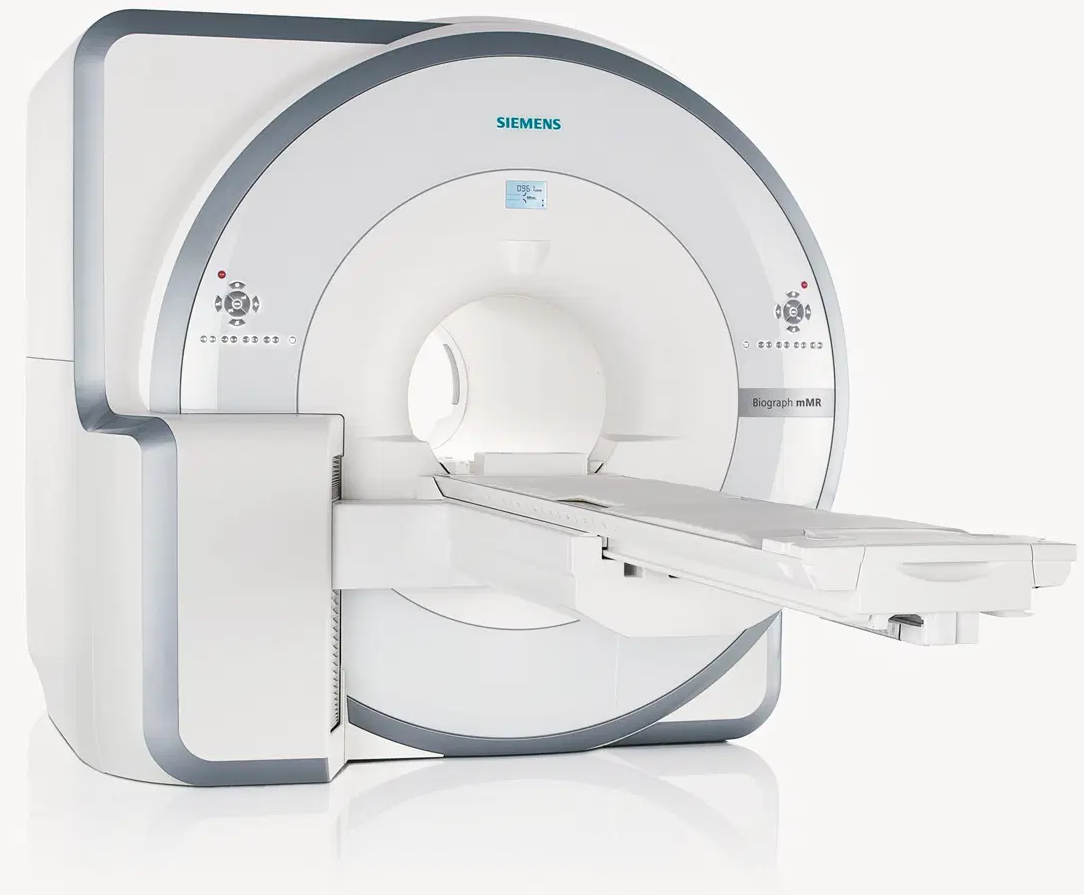
\includegraphics[width=\linewidth]{pet_machine2.png} \\ [0.5cm]
			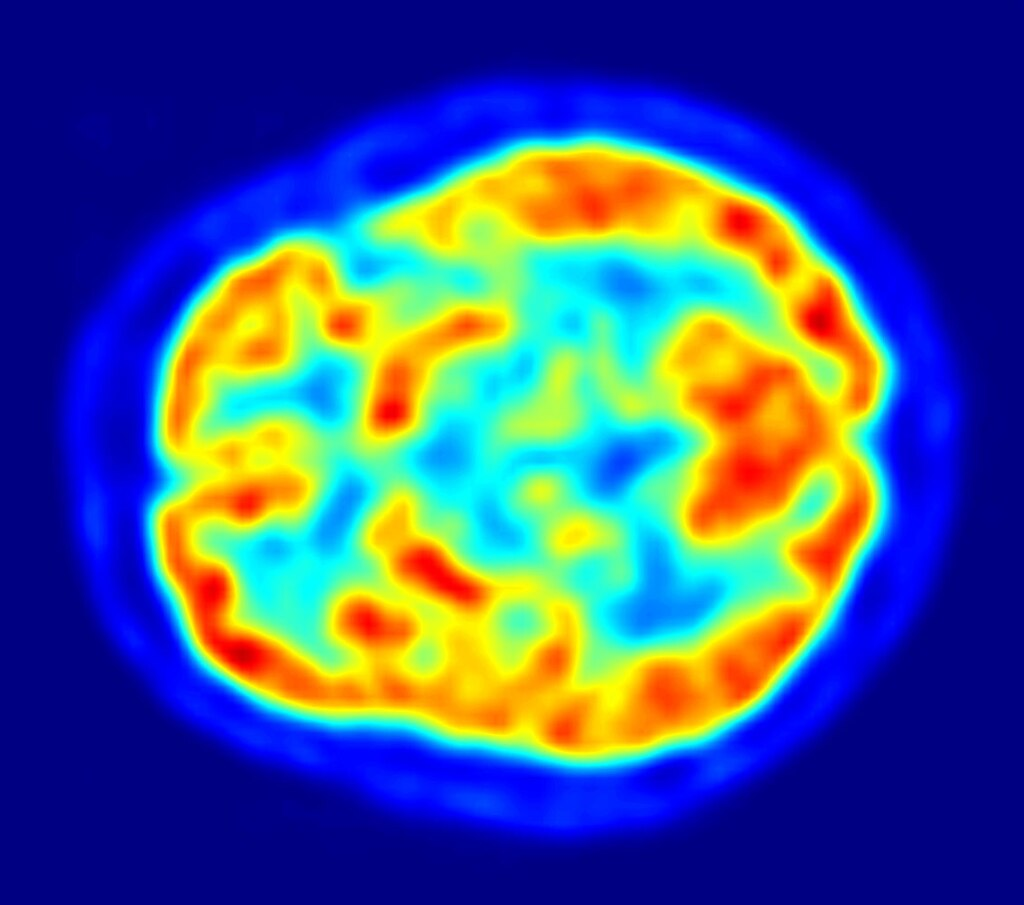
\includegraphics[width=\linewidth]{pet_image.jpg}
		\end{column}
	\end{columns}

\end{frame}

\begin{frame}[t]{Absolute Quantification in Dynamic PET}

	\begin{itemize}
		\item \textbf {Compartmental Model:} Allows for calculation of quantitative values %($\mrglu, \text{BP},\dots$)
	\end{itemize}
	\centering
	\vspace{1em}
	\begin{tikzpicture}[>=latex, thick,node distance=1.5cm, decorate]
		\node[cylinder, draw, shape border rotate=90, aspect=0.3,
			minimum height=3cm, minimum width=1.7cm,
			align=center, fill=red!80] (Cp) at (0,0) {\small Input \\ Function};

		\node[draw, rounded corners, minimum width=2.5cm, minimum height=2cm, align=center] (C1) at (4,0) {Free tracer};
		\node[draw, rounded corners, minimum width=2.5cm, minimum height=2cm, align=center] (C2) at (8,0) {Bound tracer};

		\draw[->] ([yshift=8pt]Cp.east) to[out=0, in=180] ([yshift=8pt]C1.west);
		\draw[->] ([yshift=-8pt]C1.west) to[out=180, in=0] ([yshift=-8pt]Cp.east);
		\draw[->] ([yshift=8pt]C1.east) to[out=0, in=180] ([yshift=8pt]C2.west);
		\draw[->] ([yshift=-8pt]C2.west) to[out=180, in=0] ([yshift=-8pt]C1.east);

		\begin{pgfonlayer}{background}
			\coordinate (BoxTL) at ($(C1.north west)+(-0.3,0.3)$);
			\coordinate (BoxTR) at ($(C2.north east)+(0.3,0.3)$);
			\coordinate (BoxBR) at ($(C2.south east)+(0.3,-0.3)$);
			\coordinate (BoxBL) at ($(C1.south west)+(-0.3,-0.3)$);
			\draw[dashed, rounded corners, thick, fill=yellow!40] (BoxTL) rectangle (BoxBR);
		\end{pgfonlayer}

		\node at ($(Cp.north)+(0,0.3)$) {\textbf{Blood}};
		\node at ($($(BoxTL)!0.5!(BoxTR)$)+(0,0.3)$) {\textbf{Tissue}};

		\draw[decorate,visible on=<3->, decoration={brace, mirror, amplitude=5pt,raise=0.9cm}]
		(Cp.south west) -- node[below=1.5cm] {\scalebox{2}{\Huge\color{red}{?}}} (Cp.south east);

		\draw[decorate, visible on=<2->, decoration={brace, mirror, amplitude=5pt,raise=0.5cm}]
		(BoxBL) -- node[below=1cm] {} (BoxBR);


		\begin{scope}[yshift=-5cm,visible on=<2->]
			\node at ($($(BoxBL)!0.5!(BoxBR)$)+( 0, -2)$) {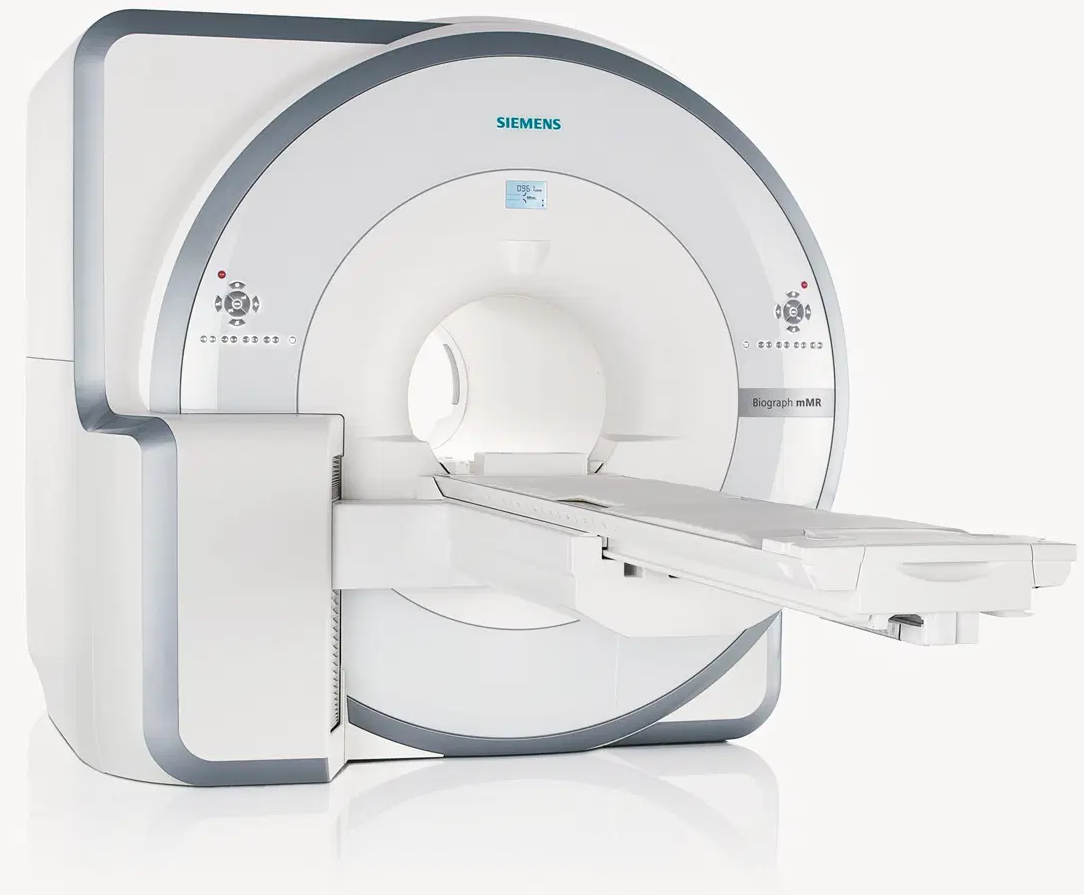
\includegraphics[height=2cm]{pet_machine2.png}};
			\node[anchor=north west,right=1cm of C2,yshift=-1cm] (ttac_image) {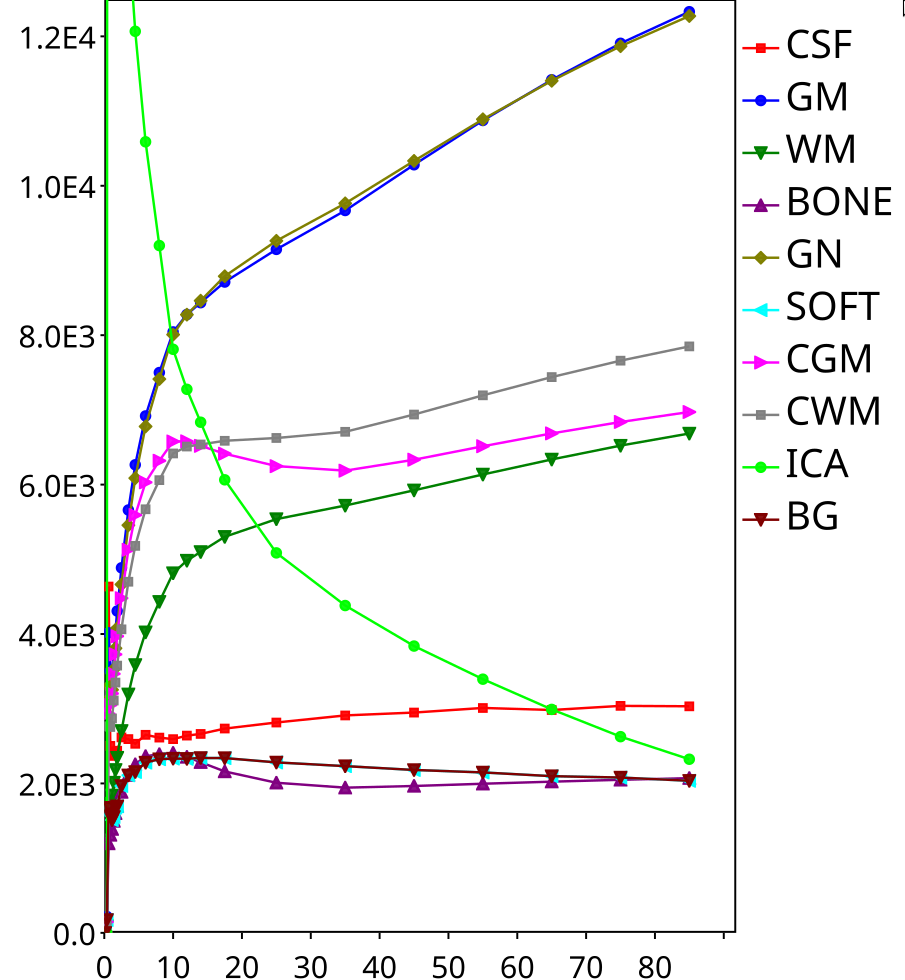
\includegraphics[width=4cm]{ttacs.png}};
			\node[above=0cm of ttac_image]{\small{Tissue Activity Curve (TAC)}};
		\end{scope}
	\end{tikzpicture}
\end{frame}

\begin{frame}{Input Function}
	\centering
	\begin{itemize}
		\item \textbf{Arterial Input Function (AIF)}: Continuous arterial sampling using a catheter
		      \begin{itemize}
			      \item The \textit{gold} standard
			      \item Invasive and uncomfortable
		      \end{itemize}
		\item \textbf{Population-Based Input Function (PBIF):} Average blood activity based on set of subjects
		\item \textbf{Image-Derived Input Function (IDIF):}
		      Direct extraction of blood radioactivity from the PET image
	\end{itemize}

	\begin{center}
		\begin{minipage}{0.40\textwidth}
			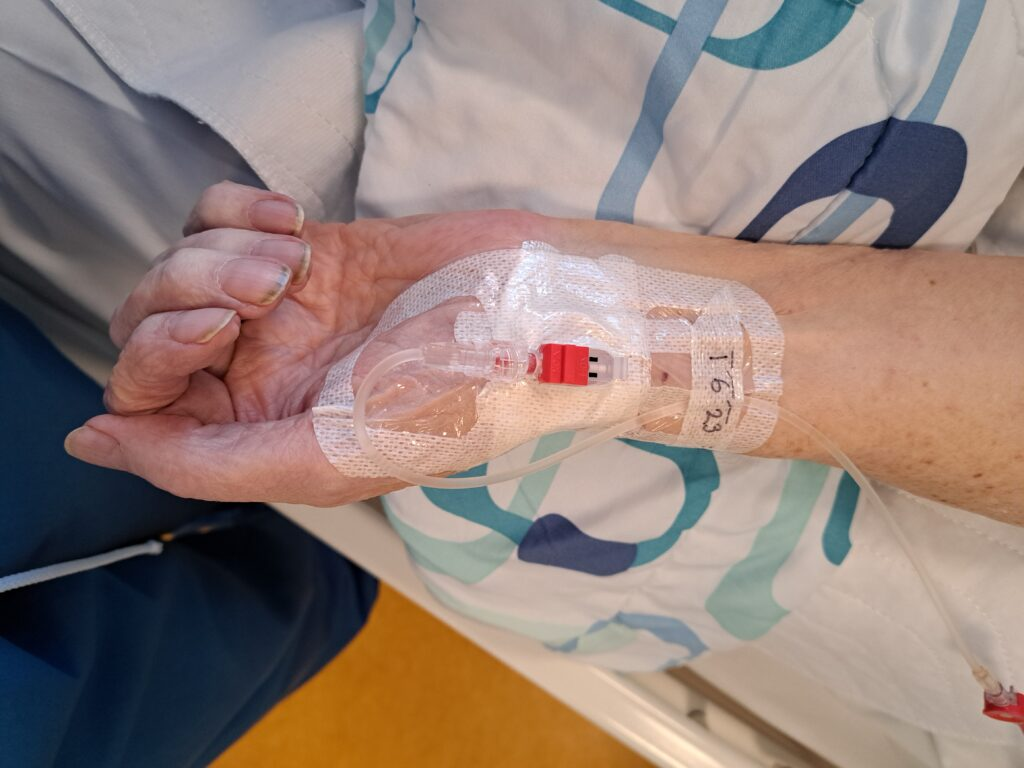
\includegraphics[width=\linewidth]{catheter2.jpg}
		\end{minipage}
		\begin{minipage}{0.40\textwidth}
			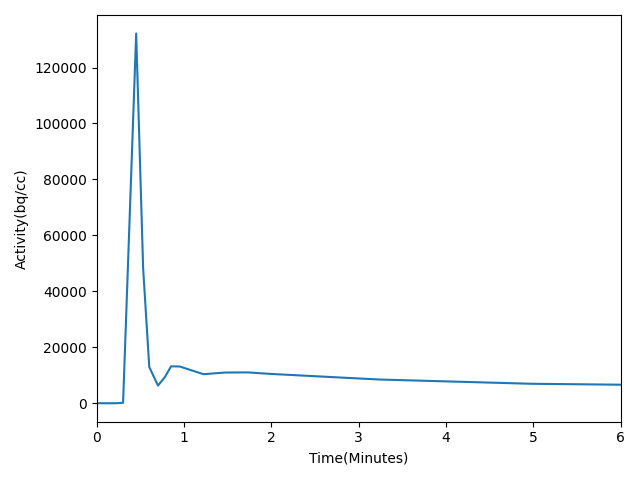
\includegraphics[width=\linewidth]{aif.png}
		\end{minipage}
		\vfill
	\end{center}

\end{frame}

\begin{frame}{How to do IDIF?}
	% \begin{enumerate}
	% 	\item Locate a major artery
	%        \item 
	% \end{enumerate}

	\begin{tikzpicture}[
			node distance=1cm,
			auto,
			>=Stealth,
			mybox/.style={draw, rounded corners, rectangle, minimum width=3cm, minimum height=1cm, align=center}
		]
		\node[mybox, visible on=<1->] (locate){Locate an Artery};
		\node[mybox, below=of locate, visible on=<1->] (mask) {Obtain an Accurate Mask};
		\node[mybox, below=of mask, visible on=<1->] (apply) {Apply to Dynamic PET};
		\node[mybox, below=of apply, sharp corners, visible on=<1->] (idif) {IDIF};

		\node[left=of mask]{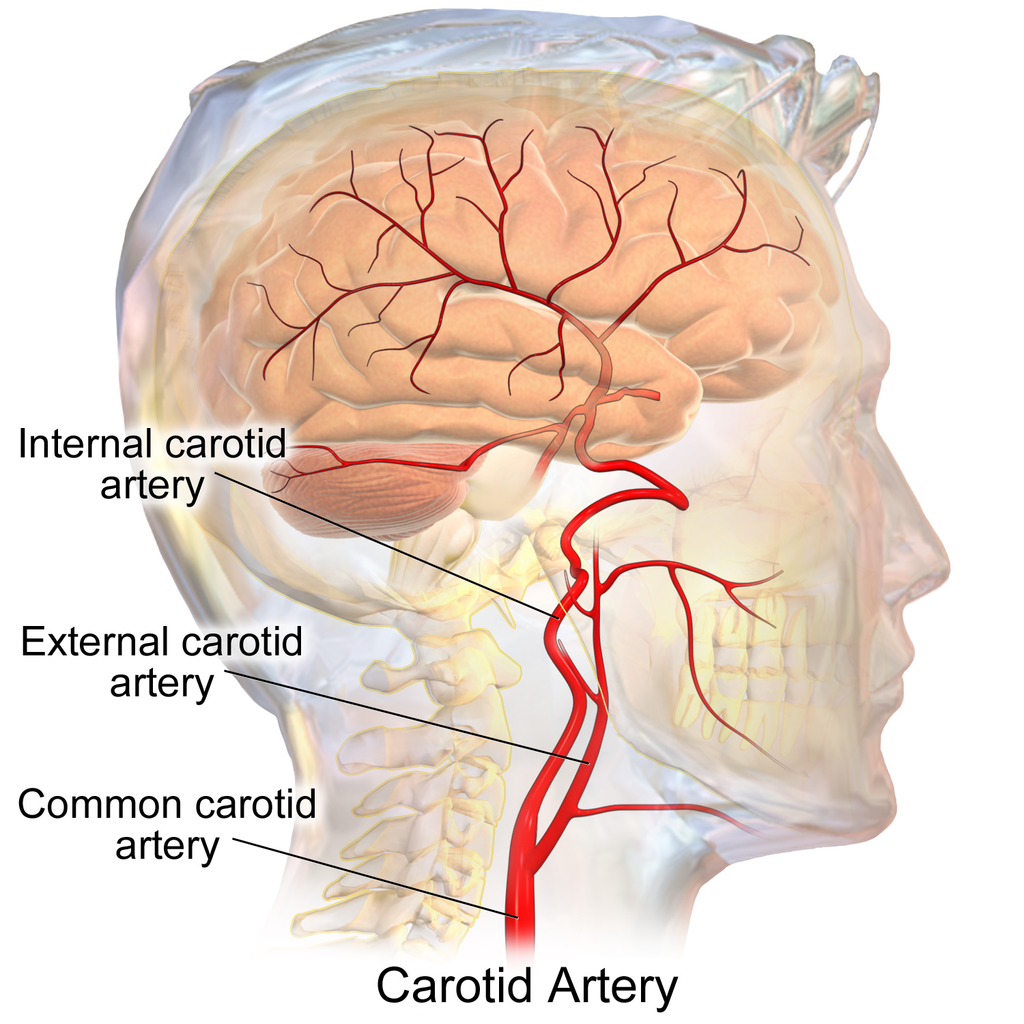
\includegraphics[width=4cm]{carotid_structure.png}};
		\node[right=of mask]{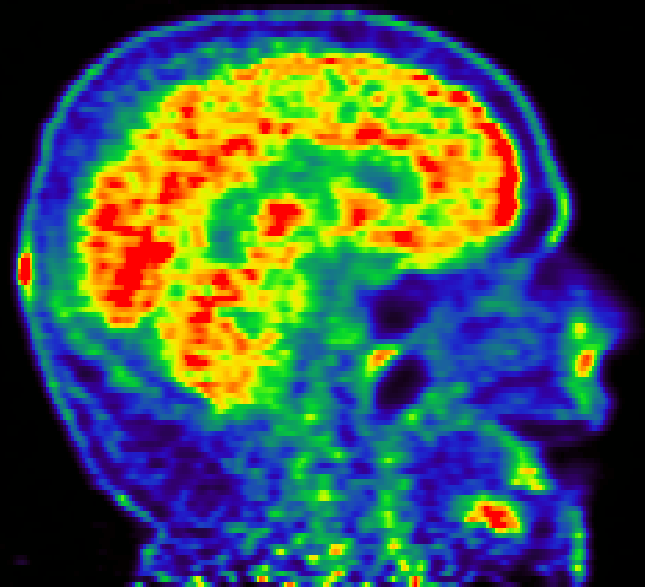
\includegraphics[width=4cm]{pet_slice_example.png}};

		\draw[->] (locate) -- (mask);
		\draw[->] (mask) -- (apply);
		\draw[->] (apply) -- (idif);
	\end{tikzpicture}
\end{frame}

% \begin{frame}{Artery Segmentation Methods}
% 	\textbf{PET Only:}
% 	\begin{itemize}
% 		\item \citeauthoryear{young2023image}: Manual delineation from early PET frames
% 		\item \citeauthoryear{}: Semi-automatic
% 		\item \citeauthoryear{chavan2024end}: Fully Automatic U-NET Network
% 	\end{itemize}
% 	\textbf{Multi-Modal:}
% 	\begin{itemize}
% 		\item \citeauthoryear{dassanayake2022caliper}
% 	\end{itemize}
% \end{frame}

\begin{frame}{Artery Segmentation Methods}
	\begin{columns}
		\small
		\begin{column}{0.7\textwidth}
			\textbf{PET Only:}
			\begin{itemize}
				\item \textbf{\citeauthoryear{young2023image}}: Manual delineation from early PET frames
				\item \textbf{\citeauthoryear{chen2007idif}}: Semi-automatic thresholding
				\item \textbf{\citeauthoryear{chavan2024end}}: Fully Automatic U-NET Network
			\end{itemize}
			\vspace{2em}
			\uncover<3->{
				\textbf{Multi-Modal:}
				\begin{itemize}
					\item \textbf{\citeauthoryear{sundar2019towards}}: Seeded region growing on TOF-MRA (semi-automatic)
					\item \textbf{\citeauthoryear{sari2017estimation}}: Fully automatic using TOF-MRA
					\item \textbf{\citeauthoryear{rahman2024deep}}: Deep learning on T1w MRI
				\end{itemize}%
			}
		\end{column}

		\begin{column}{0.3\textwidth}
			\begin{tikzpicture}[
					node distance=1cm,
					auto,
					>=Stealth,
					mybox/.style={draw, rounded corners, rectangle, minimum width=3cm, minimum height=1cm, align=center}
				]

				\node[visible on=<1>](pet){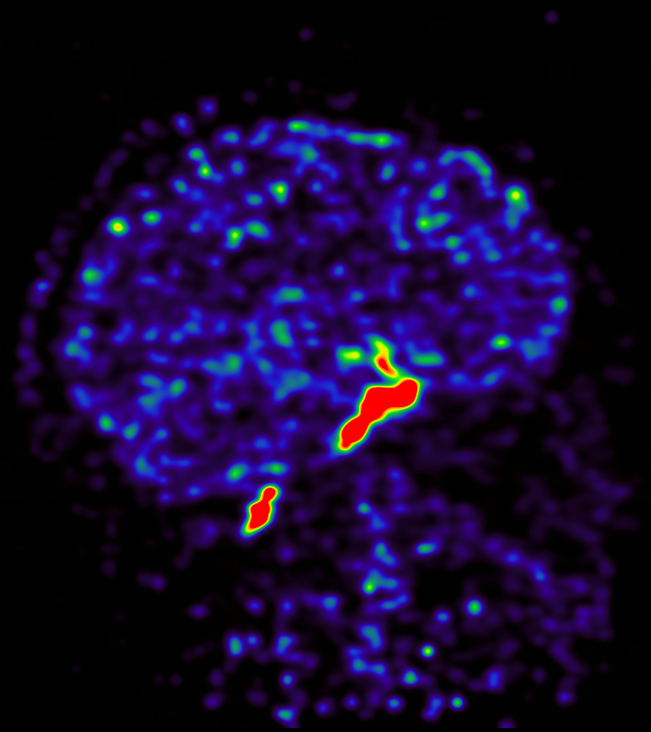
\includegraphics[height=4cm]{cpet.png}};
				\node[visible on=<2->]{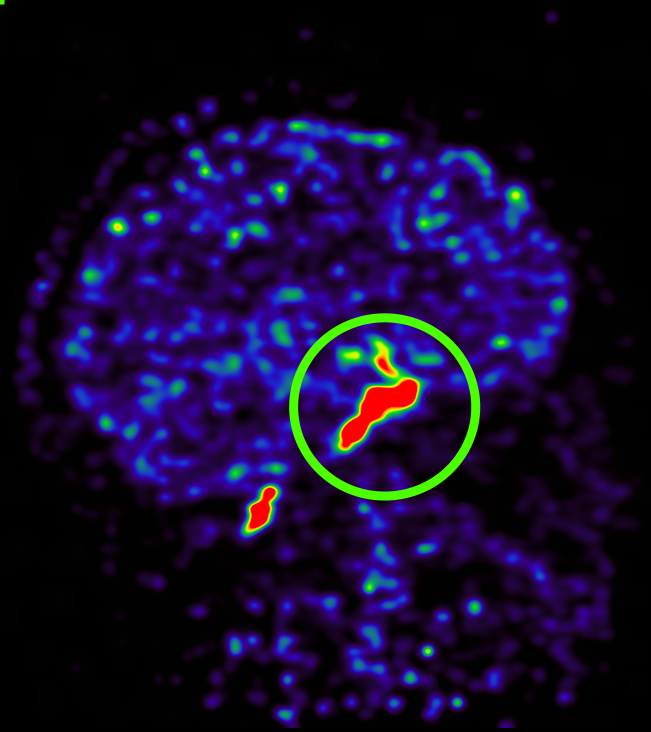
\includegraphics[height=4cm]{cpet2.png}};

				\node[below=2mm of pet, visible on=<3>](tof){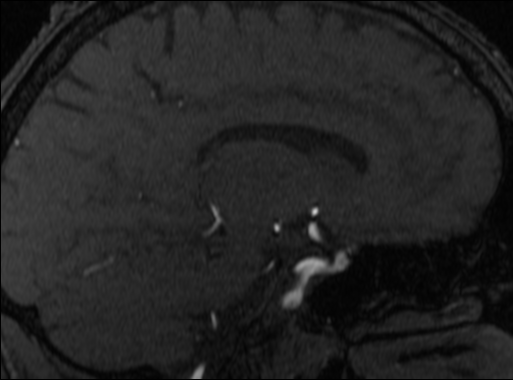
\includegraphics[height=3cm]{ctof.png}};
				\node[below=2mm of pet, visible on=<3->]{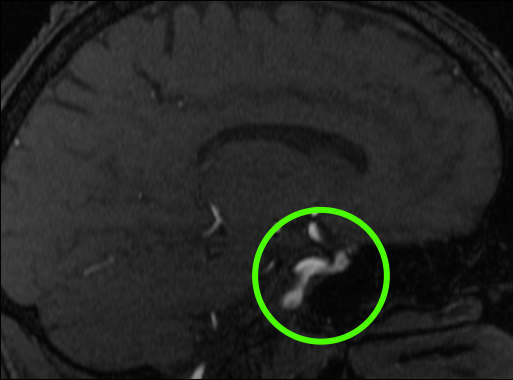
\includegraphics[height=3cm]{ctof2.png}};


				\def\tofshift{(10pt, 0pt)}
				\def\petshift{(12pt,-23pt)}

				\draw[->,bend right=15,very thick,green,visible on=<3->]
				([shift=\tofshift]tof.center) to ([shift=\petshift]pet.center);
			\end{tikzpicture}
		\end{column}
	\end{columns}
\end{frame}


\section{Methods}

\begin{frame}{Internal Carotid Artery(ICA) Segmentation Pipeline}
	\centering
	\begin{tikzpicture}[
			node distance=1.5cm,
			auto,
			>=Stealth,
			mybox/.style={draw, rounded corners, rectangle, minimum width=3cm, minimum height=1cm, align=center}
		]

		\node[mybox, alt=<2>{draw=red,very thick} ] (input) {TOF-MRA};

		\node[mybox, alt=<4>{draw=red,very thick}, visible on=<4->, right=of input, fill=yellow!20] (cuboid) { Cuboid Mask\\Application};

		\node[mybox, alt=<{3,5}>{draw=red,very thick}, right=of cuboid] (thresh) {High Intensity\\ Thresholding};
		% \node[       alt=<{3,5}>{draw=red,very thick}, above=1mm of thresh.north] (hist) {\includegraphics[width=2cm]{hist.png}};

		% \node[mybox, alt=<5>{draw=red,very thick}, right=of cuboid] (thresh2) {Adaptive Histogram\\ Thresholding};
		% \node[       alt=<5>{draw=red,very thick}, above=1mm of thresh.north] (hist2) {\includegraphics[width=2cm]{hist.png}};

		\node[mybox, alt=<5>{draw=red,very thick}, below=of thresh] (growing) {Largest 2 Volumes};
		\node[mybox, alt=<6>{draw=red,very thick}, below=of growing,fill=green] (mask) {Carotid\\Mask};
		\node[mybox, alt=<7>{draw=red,very thick}, left=of growing] (dilation) {Dilation};
		\node[mybox, alt=<7>{draw=red,very thick}, below=of dilation,fill=blue!80] (bg_mask) {Background Mask\\(surrounding tissue)};

		\node[align=center,below=1cm of input.south,visible on=<1-2>] (image) {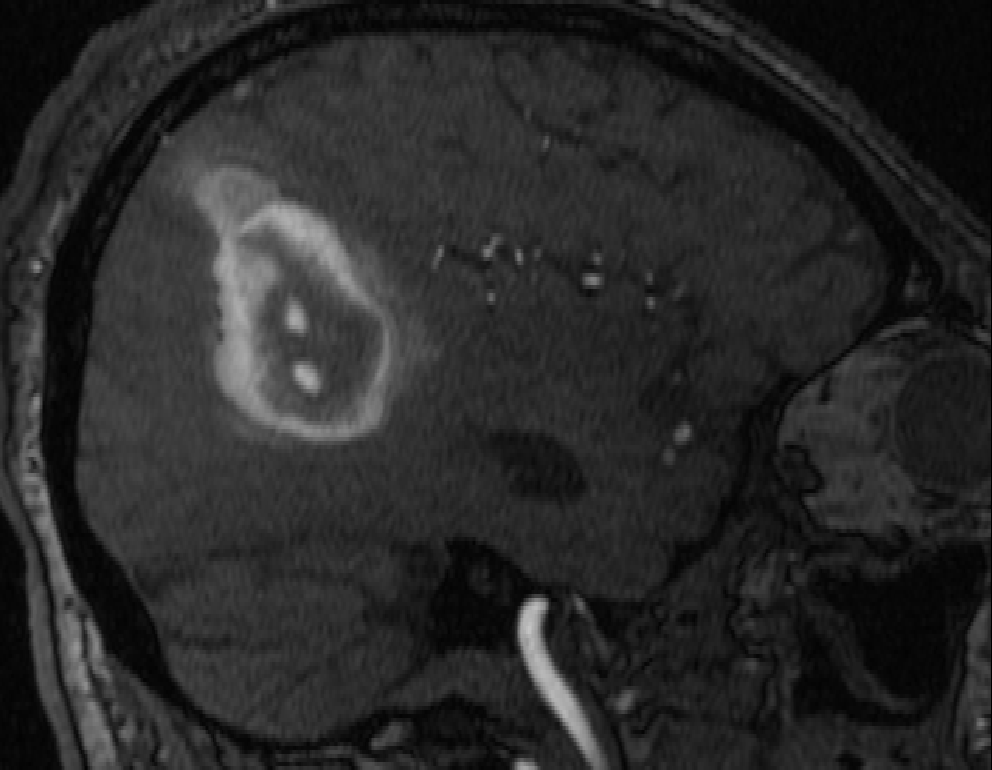
\includegraphics[width=4.5cm]{segmentation_raw.png}};
		\node[align=center,below=1cm of input.south,visible on=<3>] (image) {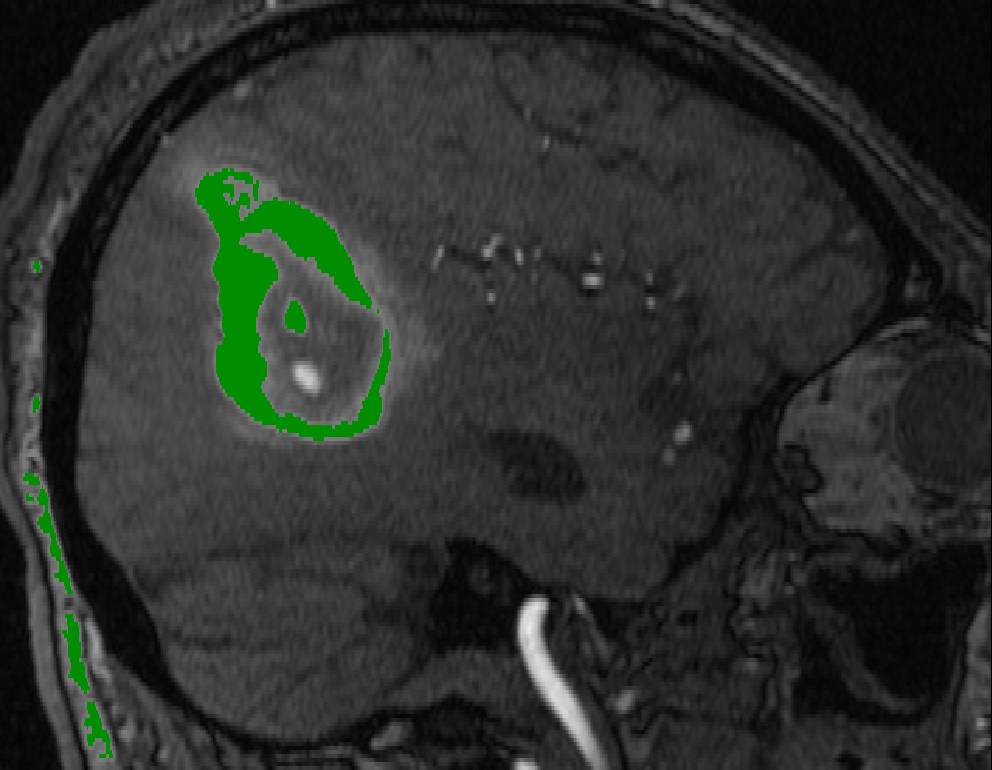
\includegraphics[width=4.5cm]{segmentation_no_bbox.png}};
		\node[align=center,below=1cm of input.south,visible on=<4>] (image) {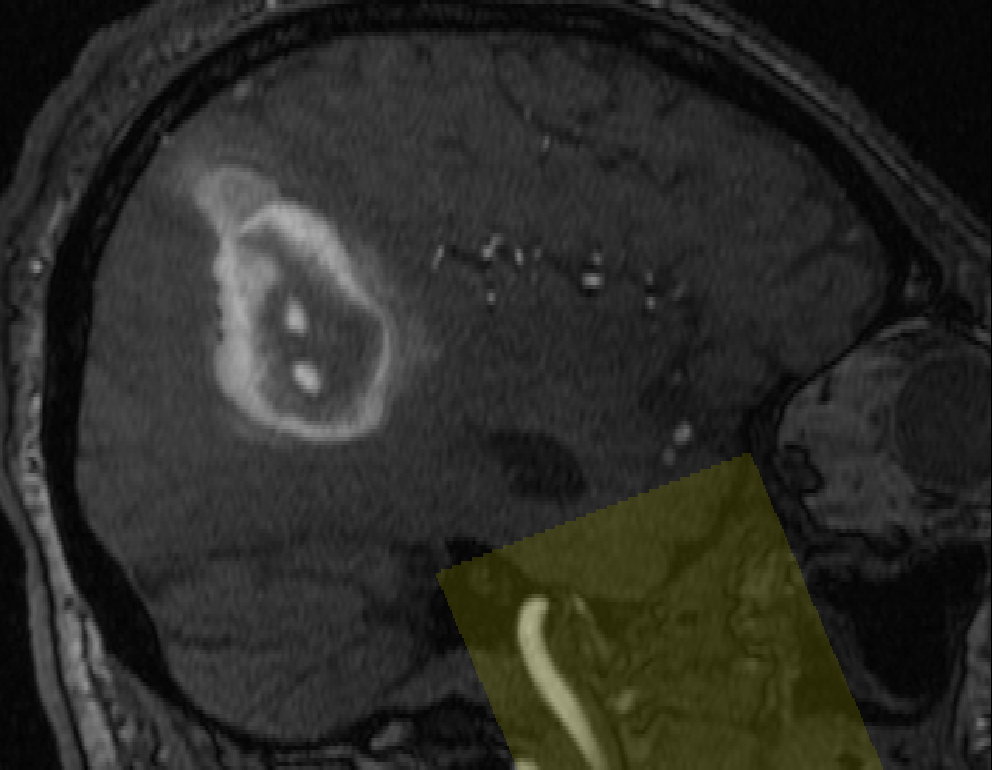
\includegraphics[width=4.5cm]{segmentation_just_bbox.png}};
		\node[align=center,below=1cm of input.south,visible on=<5-6>] (image) {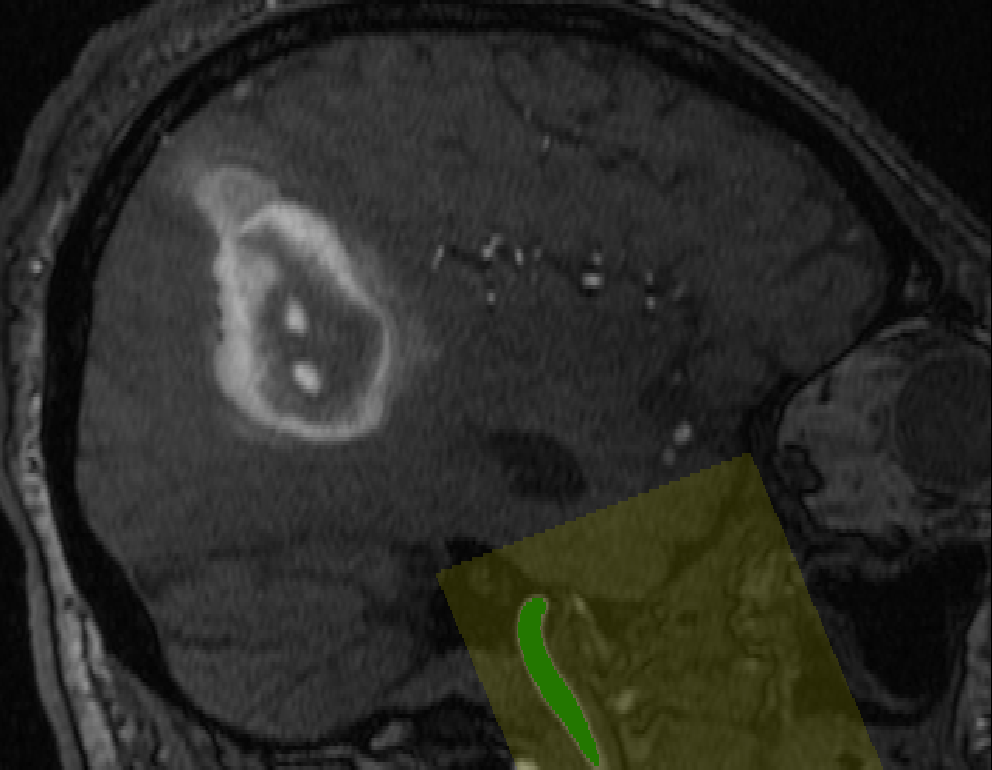
\includegraphics[width=4.5cm]{segmentation_with_bbox.png}};
		\node[align=center,below=1cm of input.south,visible on=<7->] (image) {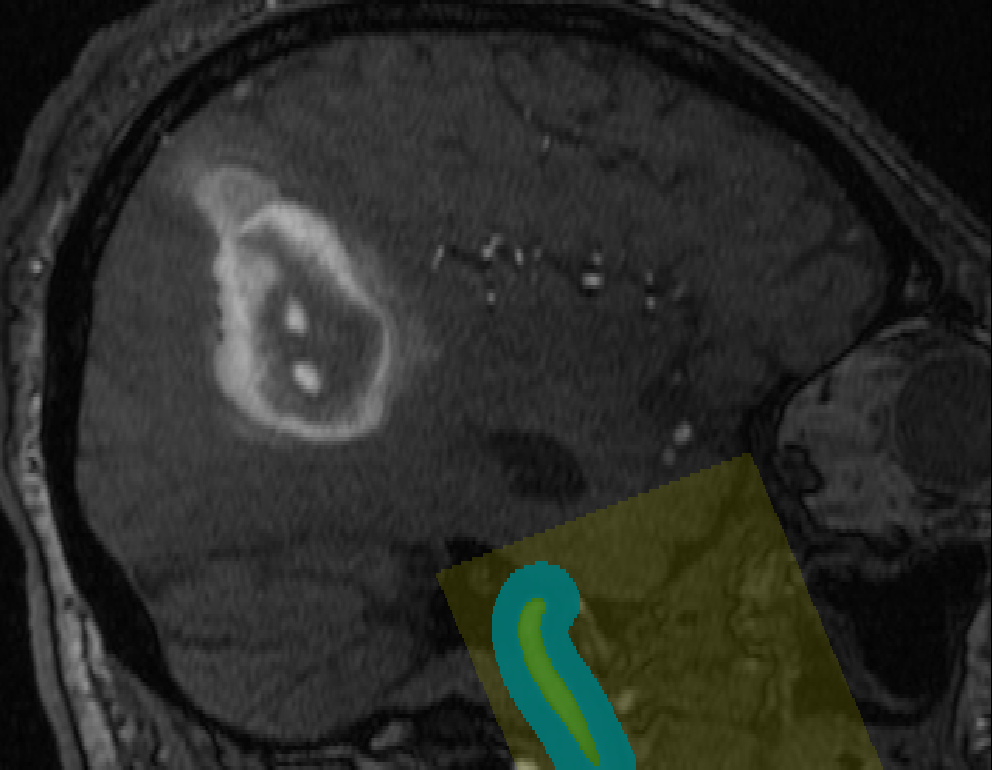
\includegraphics[width=4.5cm]{segmentation_with_bbox_and_bg.png}};


		\draw[->,visible on=<4->] (input) -- (cuboid);
		\draw[->,visible on=<4->] (cuboid) -- (thresh);
		\draw[->,visible on=<-3>] (input) -- (thresh);

		\draw[->] (thresh) -- (growing);
		\draw[->] (growing) -- (mask);
		\draw[->] (growing) -- (dilation);
		\draw[->] (dilation) -- (bg_mask);

	\end{tikzpicture}
\end{frame}

% \begin{frame}[t]{IDIF Challenges:}
% 	\textbf{1) Segmentation:} A vessel must be accurately segmented to extract the input function from the PET
% 	\vfill
% 	\textbf{2) Partial Volume Effect:} Signals mix with surrounding tissues (Spill-in \& Spill-out).
%
% 	\begin{center}
% 		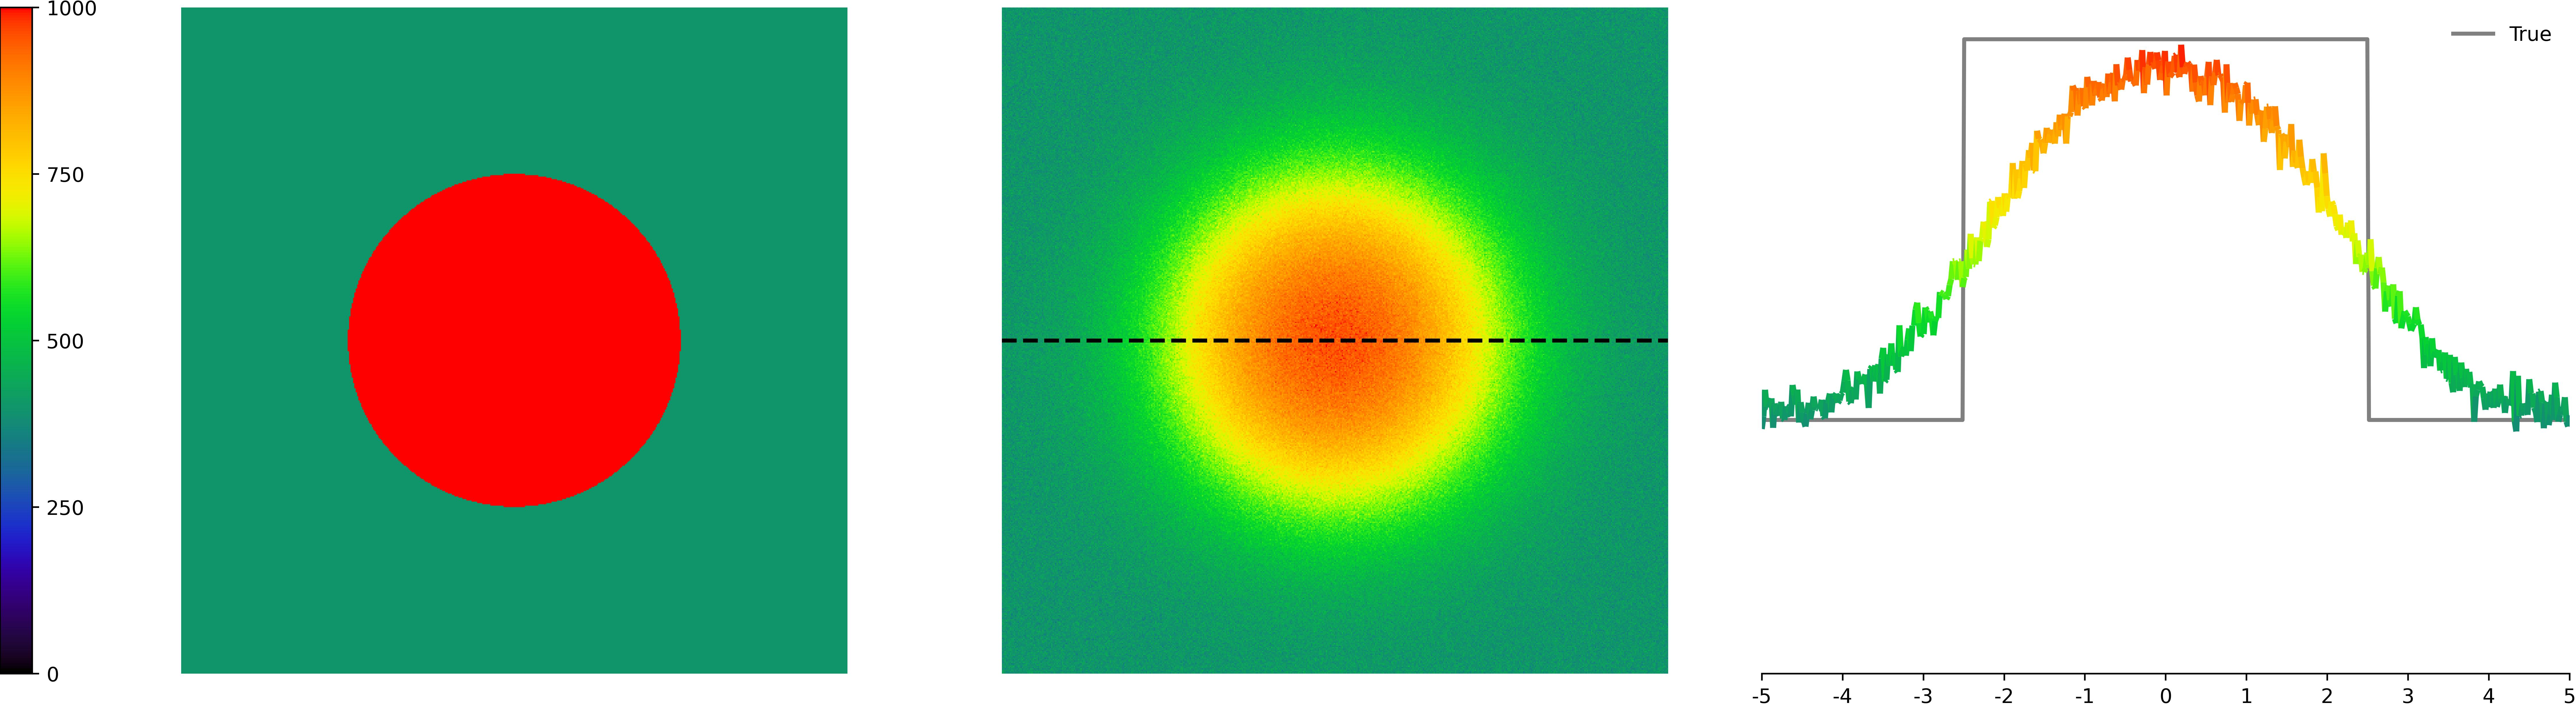
\includegraphics[width=0.9\textwidth]{pve.jpg}
% 	\end{center}
% \end{frame}

\begin{frame}{Image Derived Input Function (IDIF)}
	\resizebox{0.95\textwidth}{!}{%
		\begin{tikzpicture}[
				node distance=1cm,
				auto,
				>=Stealth,
				mybox/.style={draw, rounded corners, rectangle, minimum width=3cm, minimum height=1cm, align=center}
			]
			\node[mybox] (mri) {MR Angiography};
			\node[mybox,right=of mri] (artery) {Artery Mask};
			\node[mybox,below=of artery] (pet) {Dynamic PET};
			% \coordinate (mid) at ($(artery)!0.5!(pet)$);
			\node[mybox,right=3 of pet](idif){Image Derived\\Input Function};
			\node[above=0cm of mri,visible on=<1>]{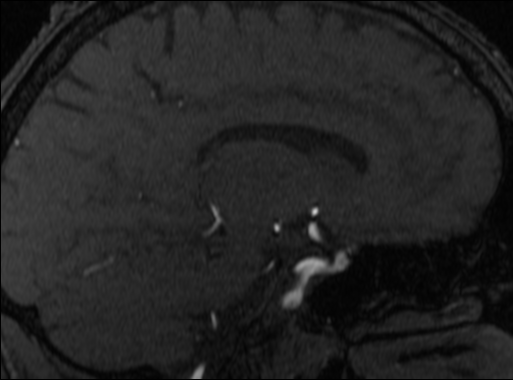
\includegraphics[height=2.5cm]{ctof.png}};
			\node[above=0cm of mri,visible on=<2->]{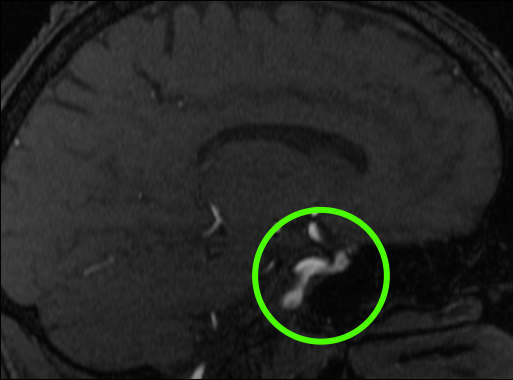
\includegraphics[height=2.5cm]{ctof2.png}};

			\node[below=0cm of mri,visible on=<1>]{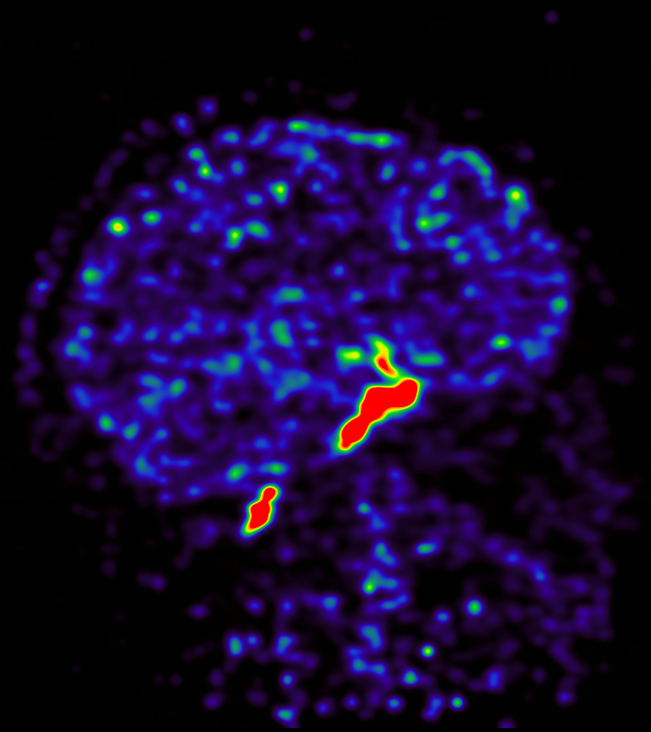
\includegraphics[height=2.5cm]{cpet.png}};
			\node[below=0cm of mri,visible on=<2->]{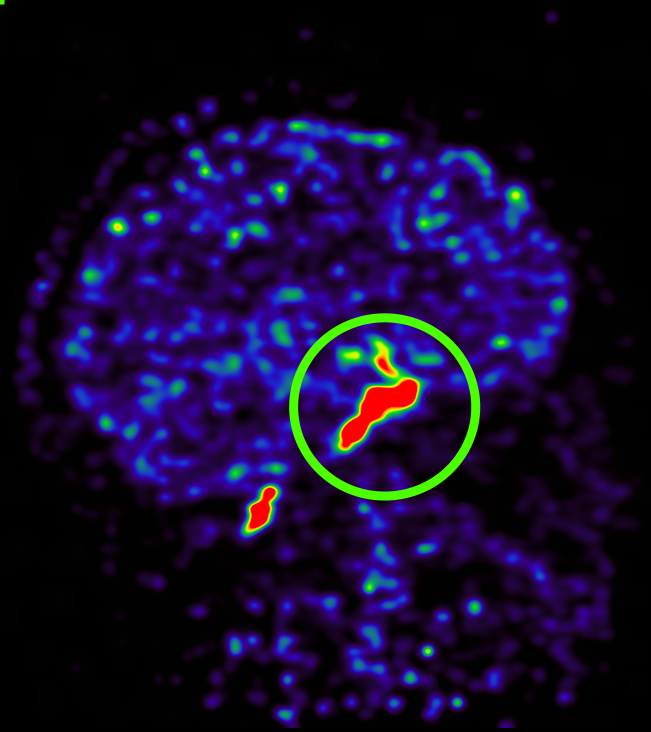
\includegraphics[height=2.5cm]{cpet2.png}};
			\node[above=0cm of artery,visible on=<2->]{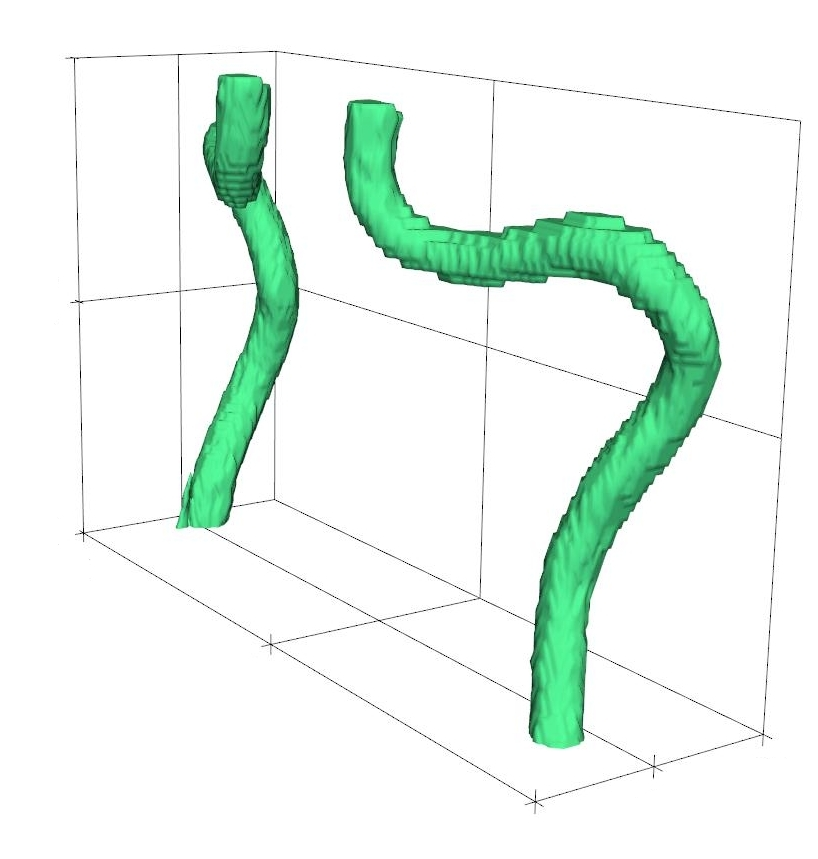
\includegraphics[height=2.5cm]{carotid_3d.jpg}};

			\node[anchor=south west,visible on=<3->] at($(pet.north east)+(1.2,0)$) {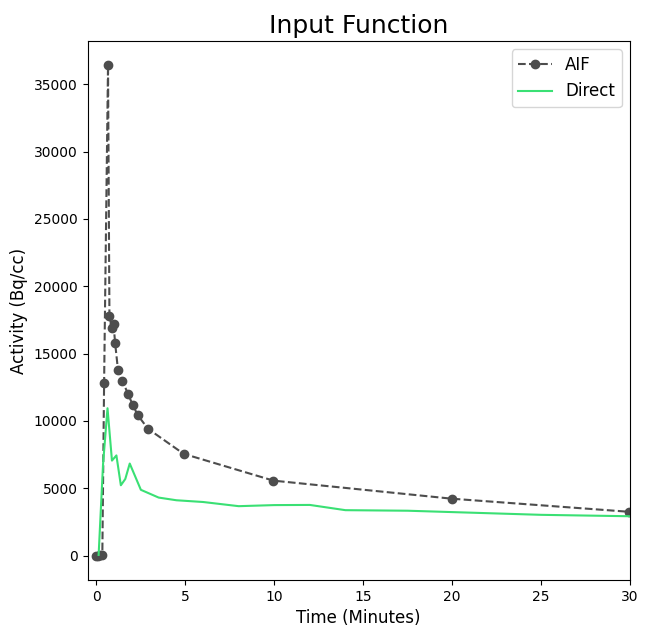
\includegraphics[width=6cm]{BADKA07504_1_infunc_direct2.png}};

			\draw[->] (mri.east) -- (artery.west);
			\draw[->] (artery.east) to[out=0, in=180] (idif.west);
			\draw[->] (pet.east) to[out=0, in=180] (idif.west);
		\end{tikzpicture}% 
	}
\end{frame}


\begin{frame}{Partial Volume Effect}
	\begin{center}
		\Large\textbf{Mixture of Activity with surrounding tissues\\(Spill-in \& Spill-out Effects)}

		% 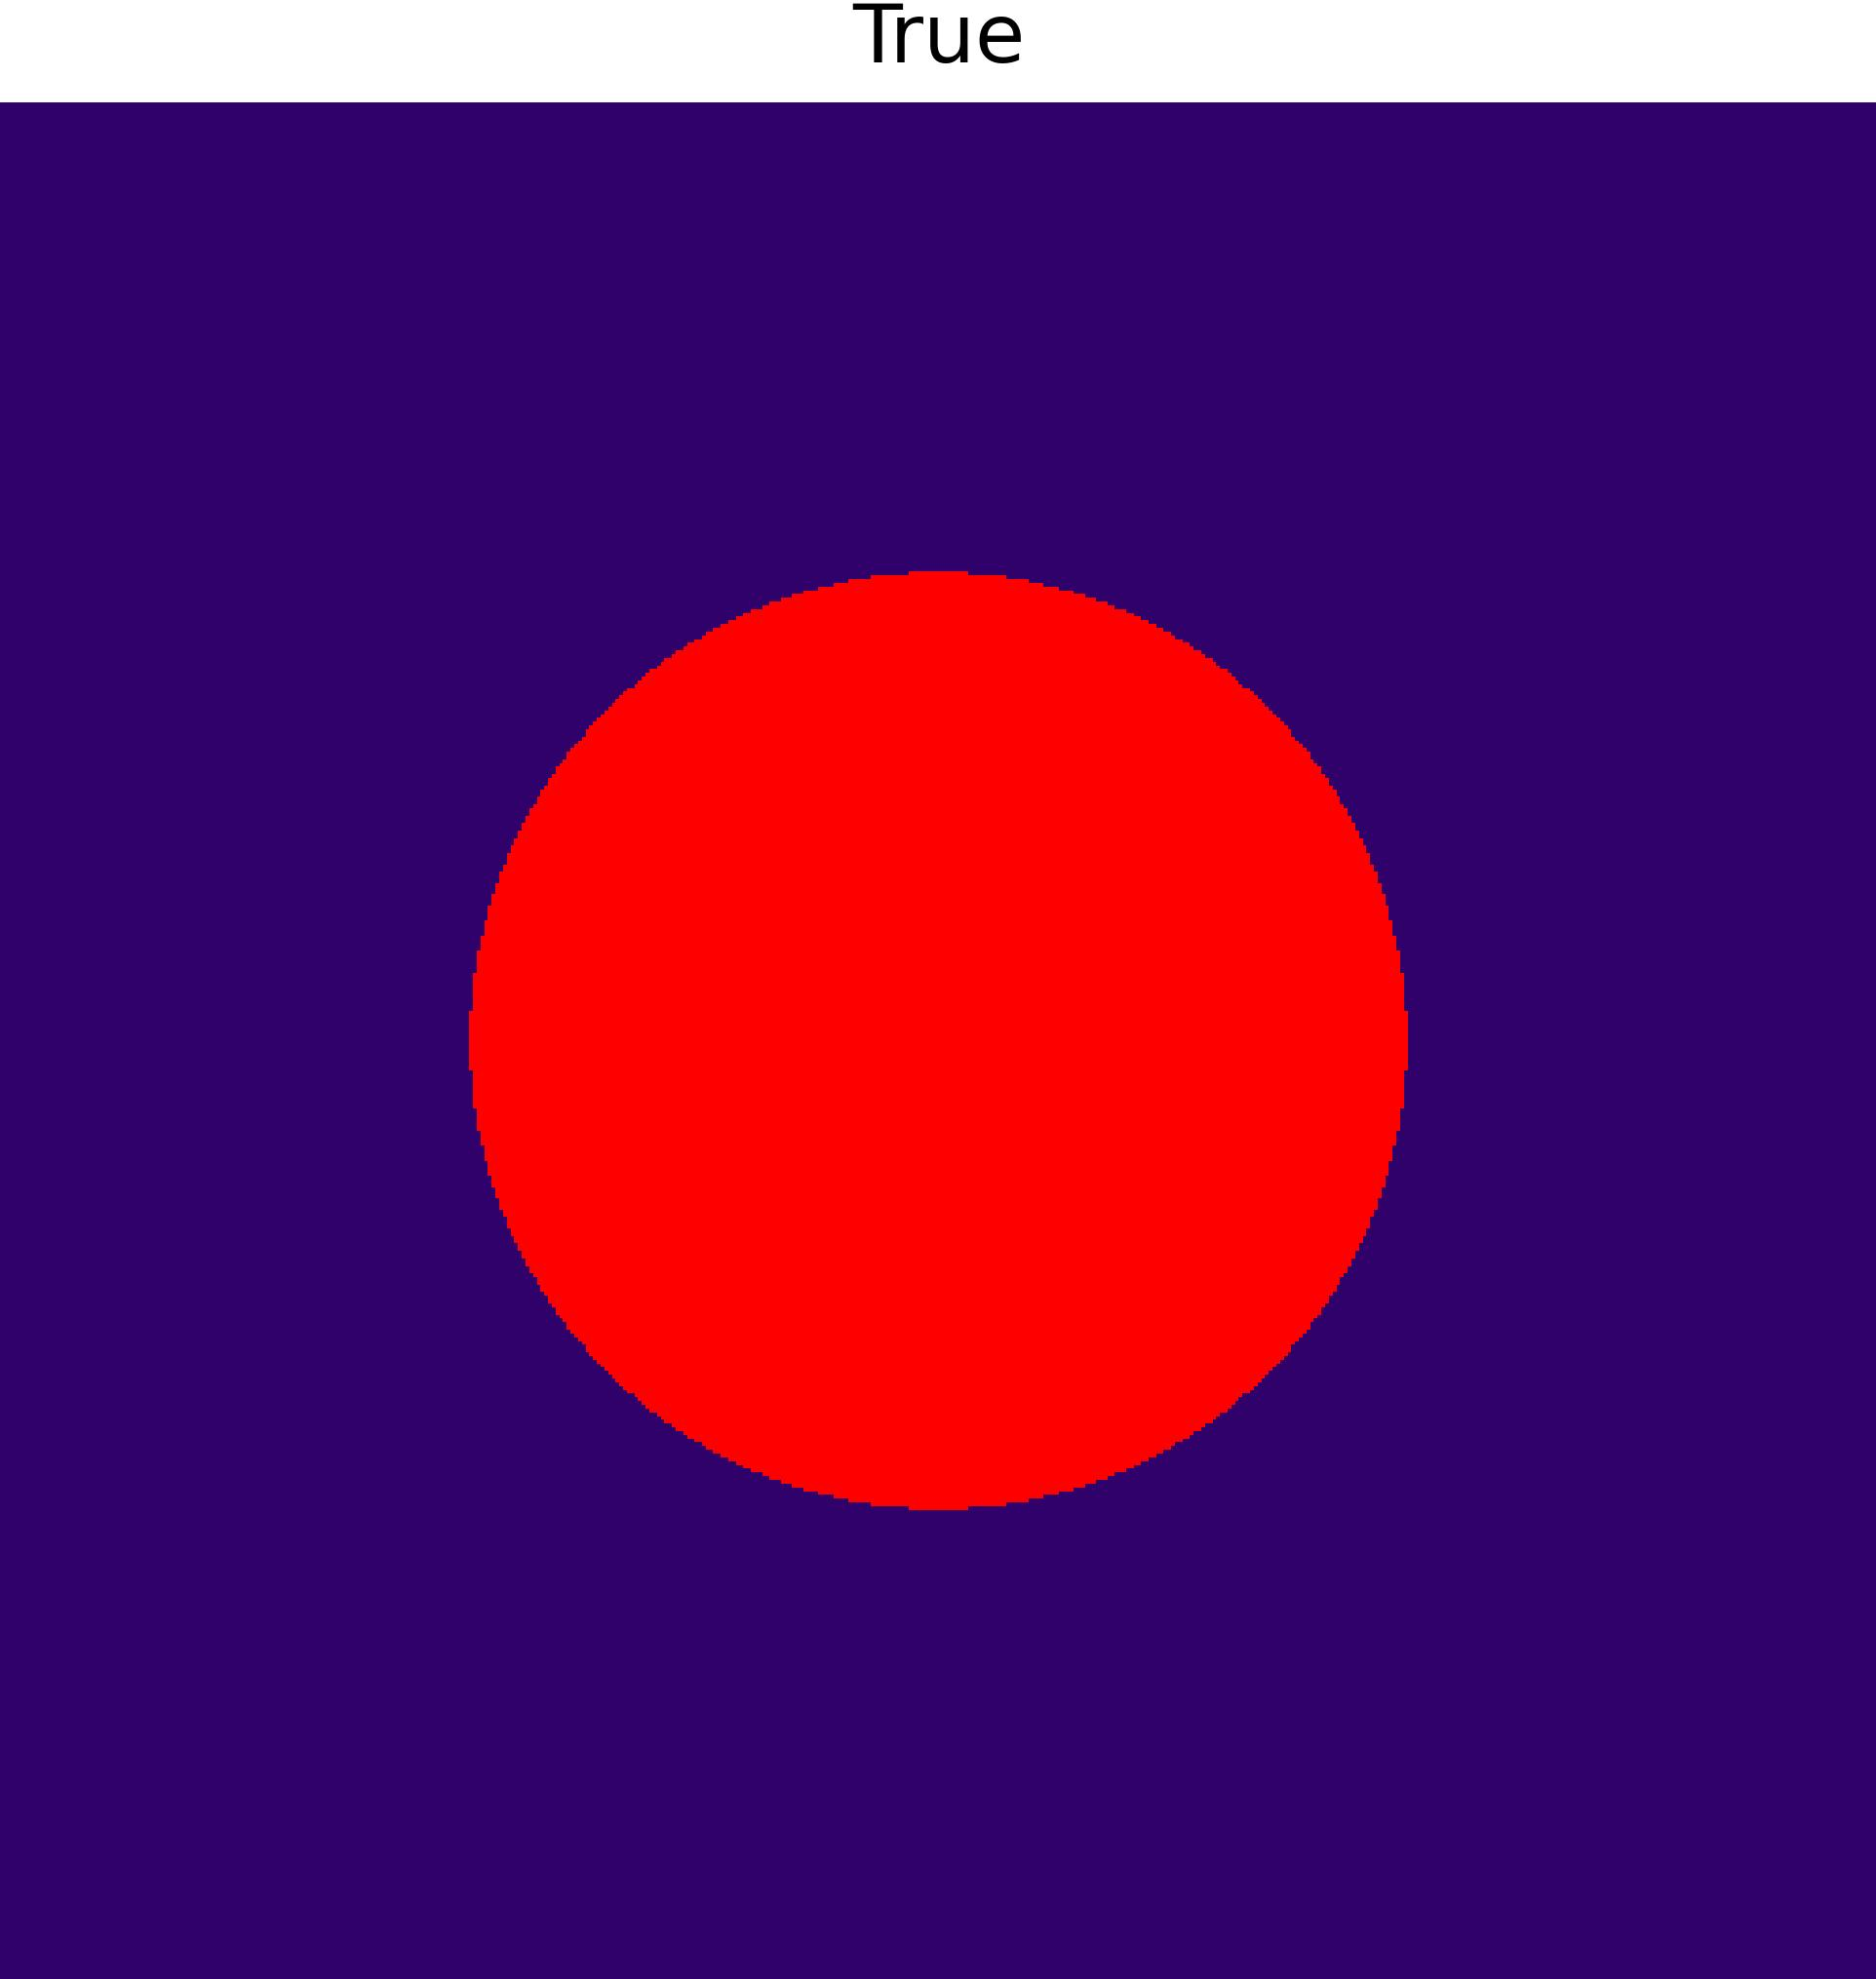
\includegraphics[height=5cm]{pve_true.jpg}
		\vfill
		\begin{tikzpicture}
			\node[anchor=north west, inner sep=0] (img)
			at (0,0) {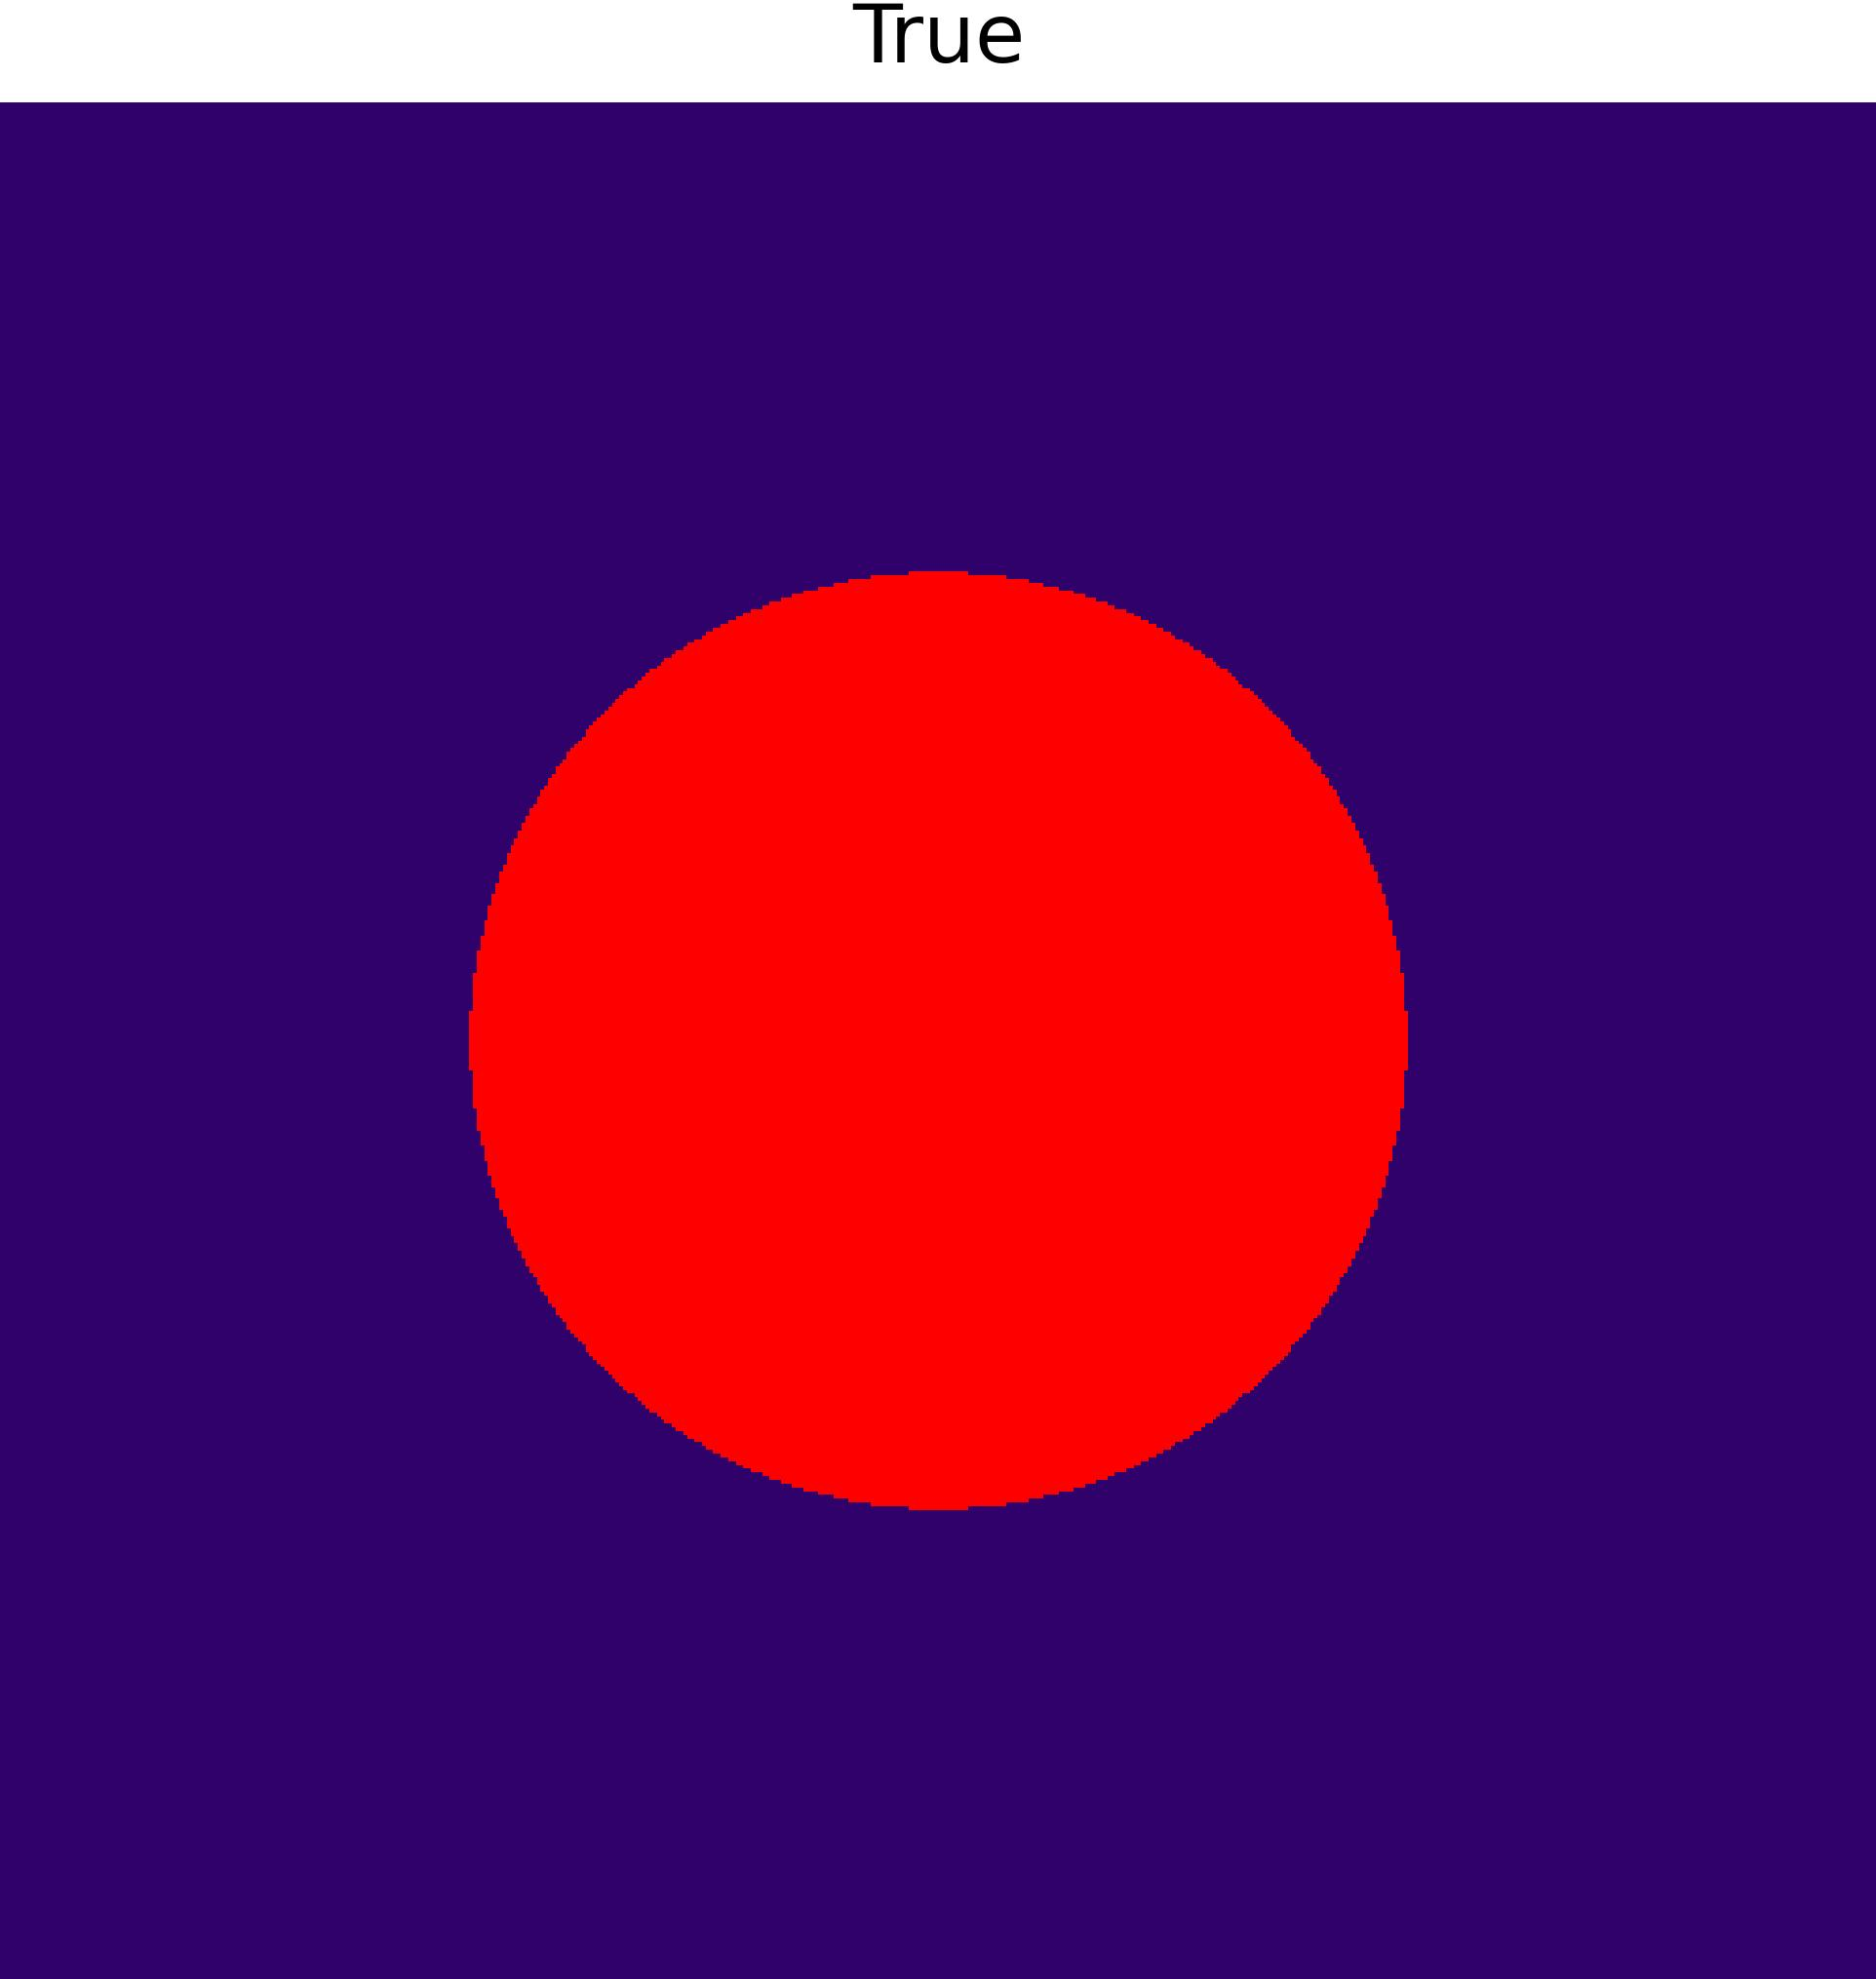
\includegraphics[height=5cm]{pve_true.jpg}};
			% \begin{scope}[x={(img.north east)}, y={(img.south west)},visible on=<2->]
			% 	\draw[->, >=stealth, bend left=30,thick, color=white]
			% 	(0.6,0.47) to node[above, text=white] {\small $\omega_{out}$} (0.85,0.47);
			% 	\draw[<-, >=stealth, bend right=30,thick, color=white]
			% 	(0.6,0.57) to node[below, text=white] {\small $\omega_{in}$} (0.85,0.57);
			% \end{scope}
		\end{tikzpicture}
		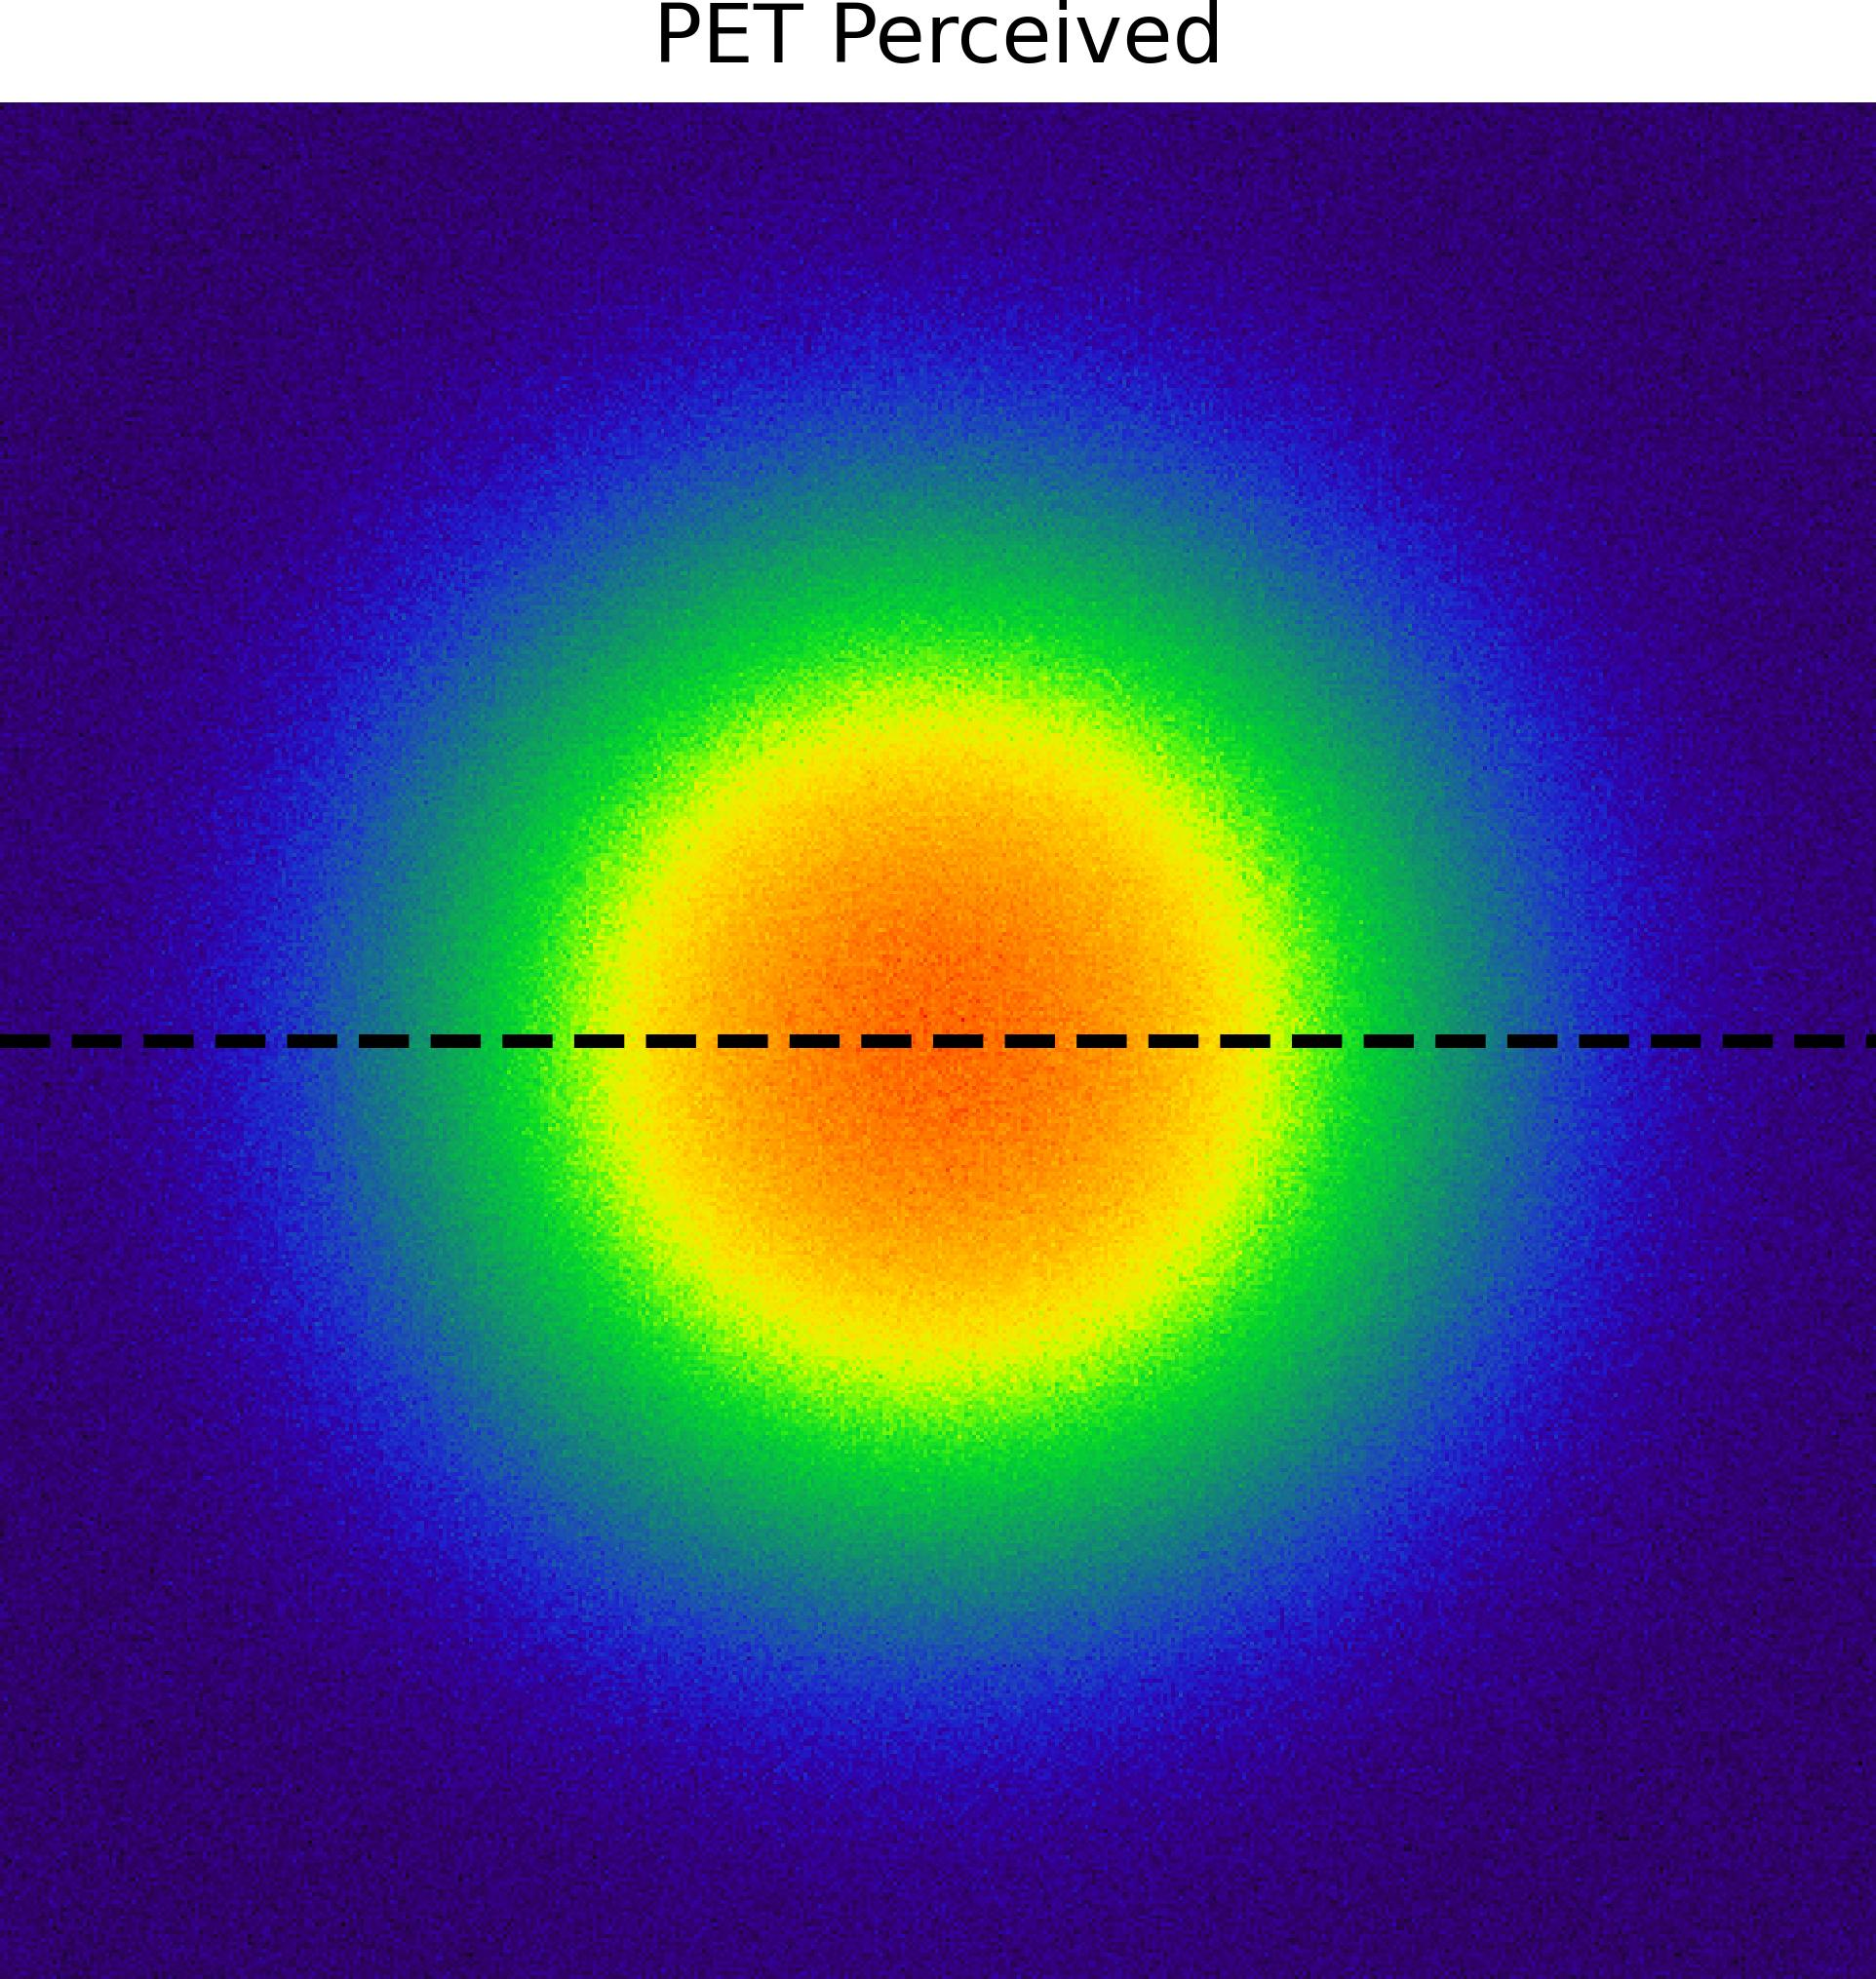
\includegraphics[height=5cm]{pve_perceived.jpg}
		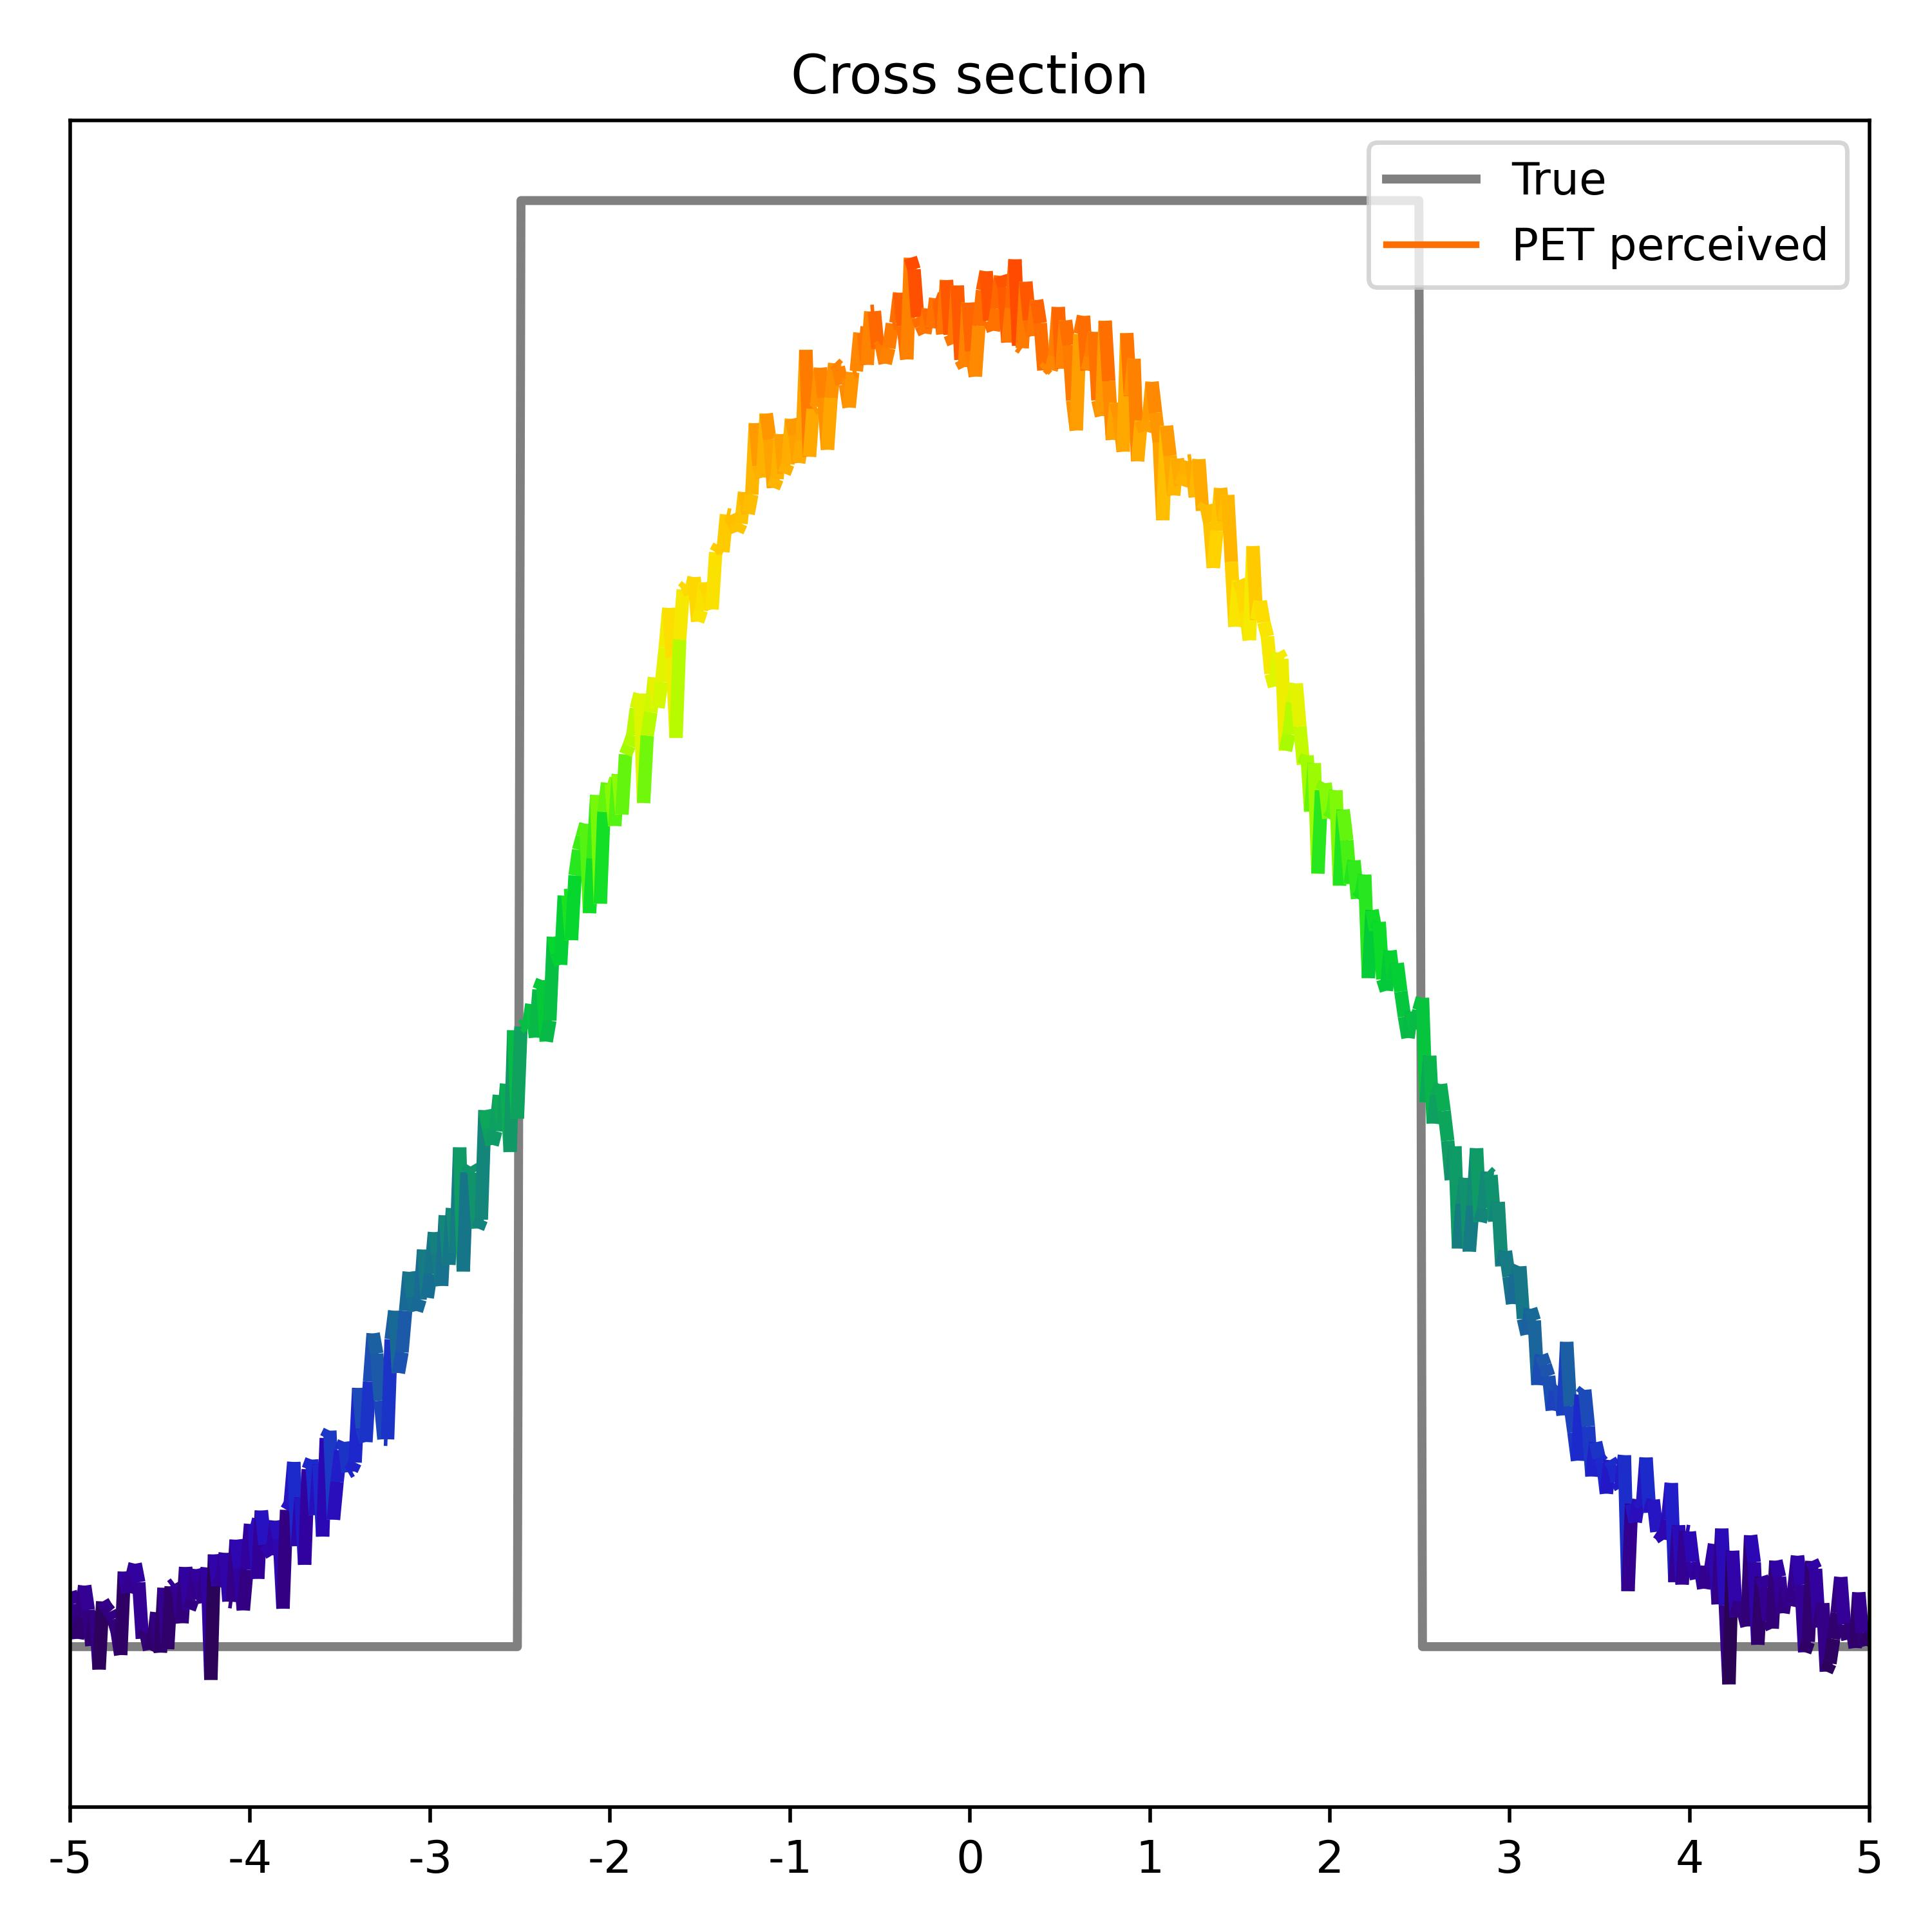
\includegraphics[height=5cm]{pve_crosssection.jpg}
	\end{center}
\end{frame}

\begin{frame}[t]{Partial Volume Correction(PVC)}
	\begin{columns}
		\begin{column}{0.7\textwidth}
			\small
			\begin{itemize}
				\setlength\itemsep{2em}
				\item Recovery Coefficient (RC): Spillage coefficients dervied from cylindrical phantoms
				\item Deep learning models
				\item Geometric Transfer Matrix (GTM)
				\item ...
			\end{itemize}
		\end{column}
		\begin{column}{0.3\textwidth}
			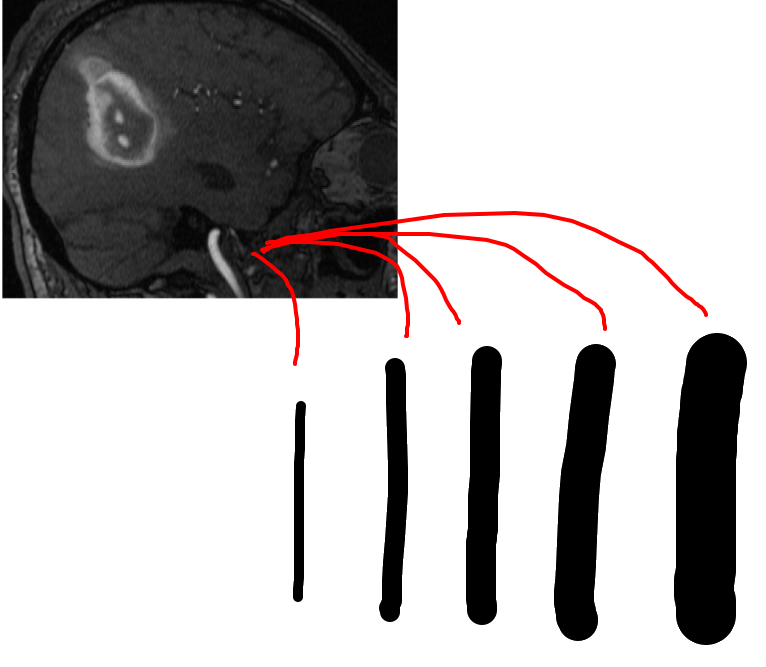
\includegraphics[width=\linewidth]{rc.png}
			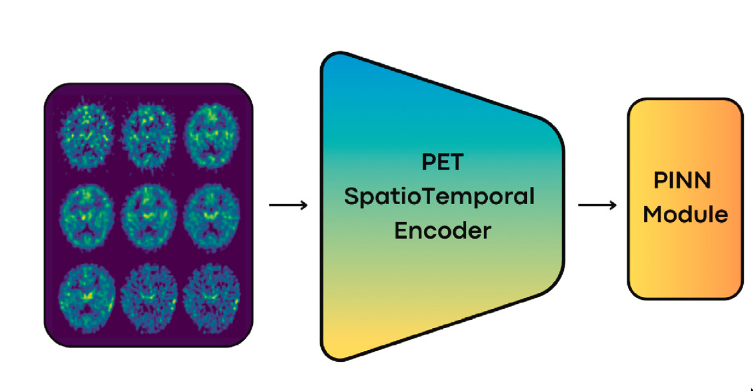
\includegraphics[width=\linewidth]{cnn.png}
		\end{column}
	\end{columns}
\end{frame}
\begin{frame}{Geometric Transfer Matrix (GTM)}
	Linear combination of the true Time Activity Curve (TAC) with the other effecting regions
	\begin{equation*}
		\underbrace{
			\begin{bmatrix}
				T_{c} \\
				T_{bg}
			\end{bmatrix}
		}_{\text{Observered}}
		=
		\underbrace{
			\begin{bmatrix}
				\omega_{c \rightarrow c}  & \omega_{bg \rightarrow c}  \\
				\omega_{c \rightarrow bg} & \omega_{bg \rightarrow bg}
			\end{bmatrix}
		}_{\text{GTM}}
		.
		\underbrace{
			\begin{bmatrix}
				T_{IF} \\
				T_{tissue}
			\end{bmatrix}
		}_{\text{Unknown}}
	\end{equation*}

	\centering
	\begin{tikzpicture}
		\node[anchor=north west, inner sep=0] (img)
		at (0,0) {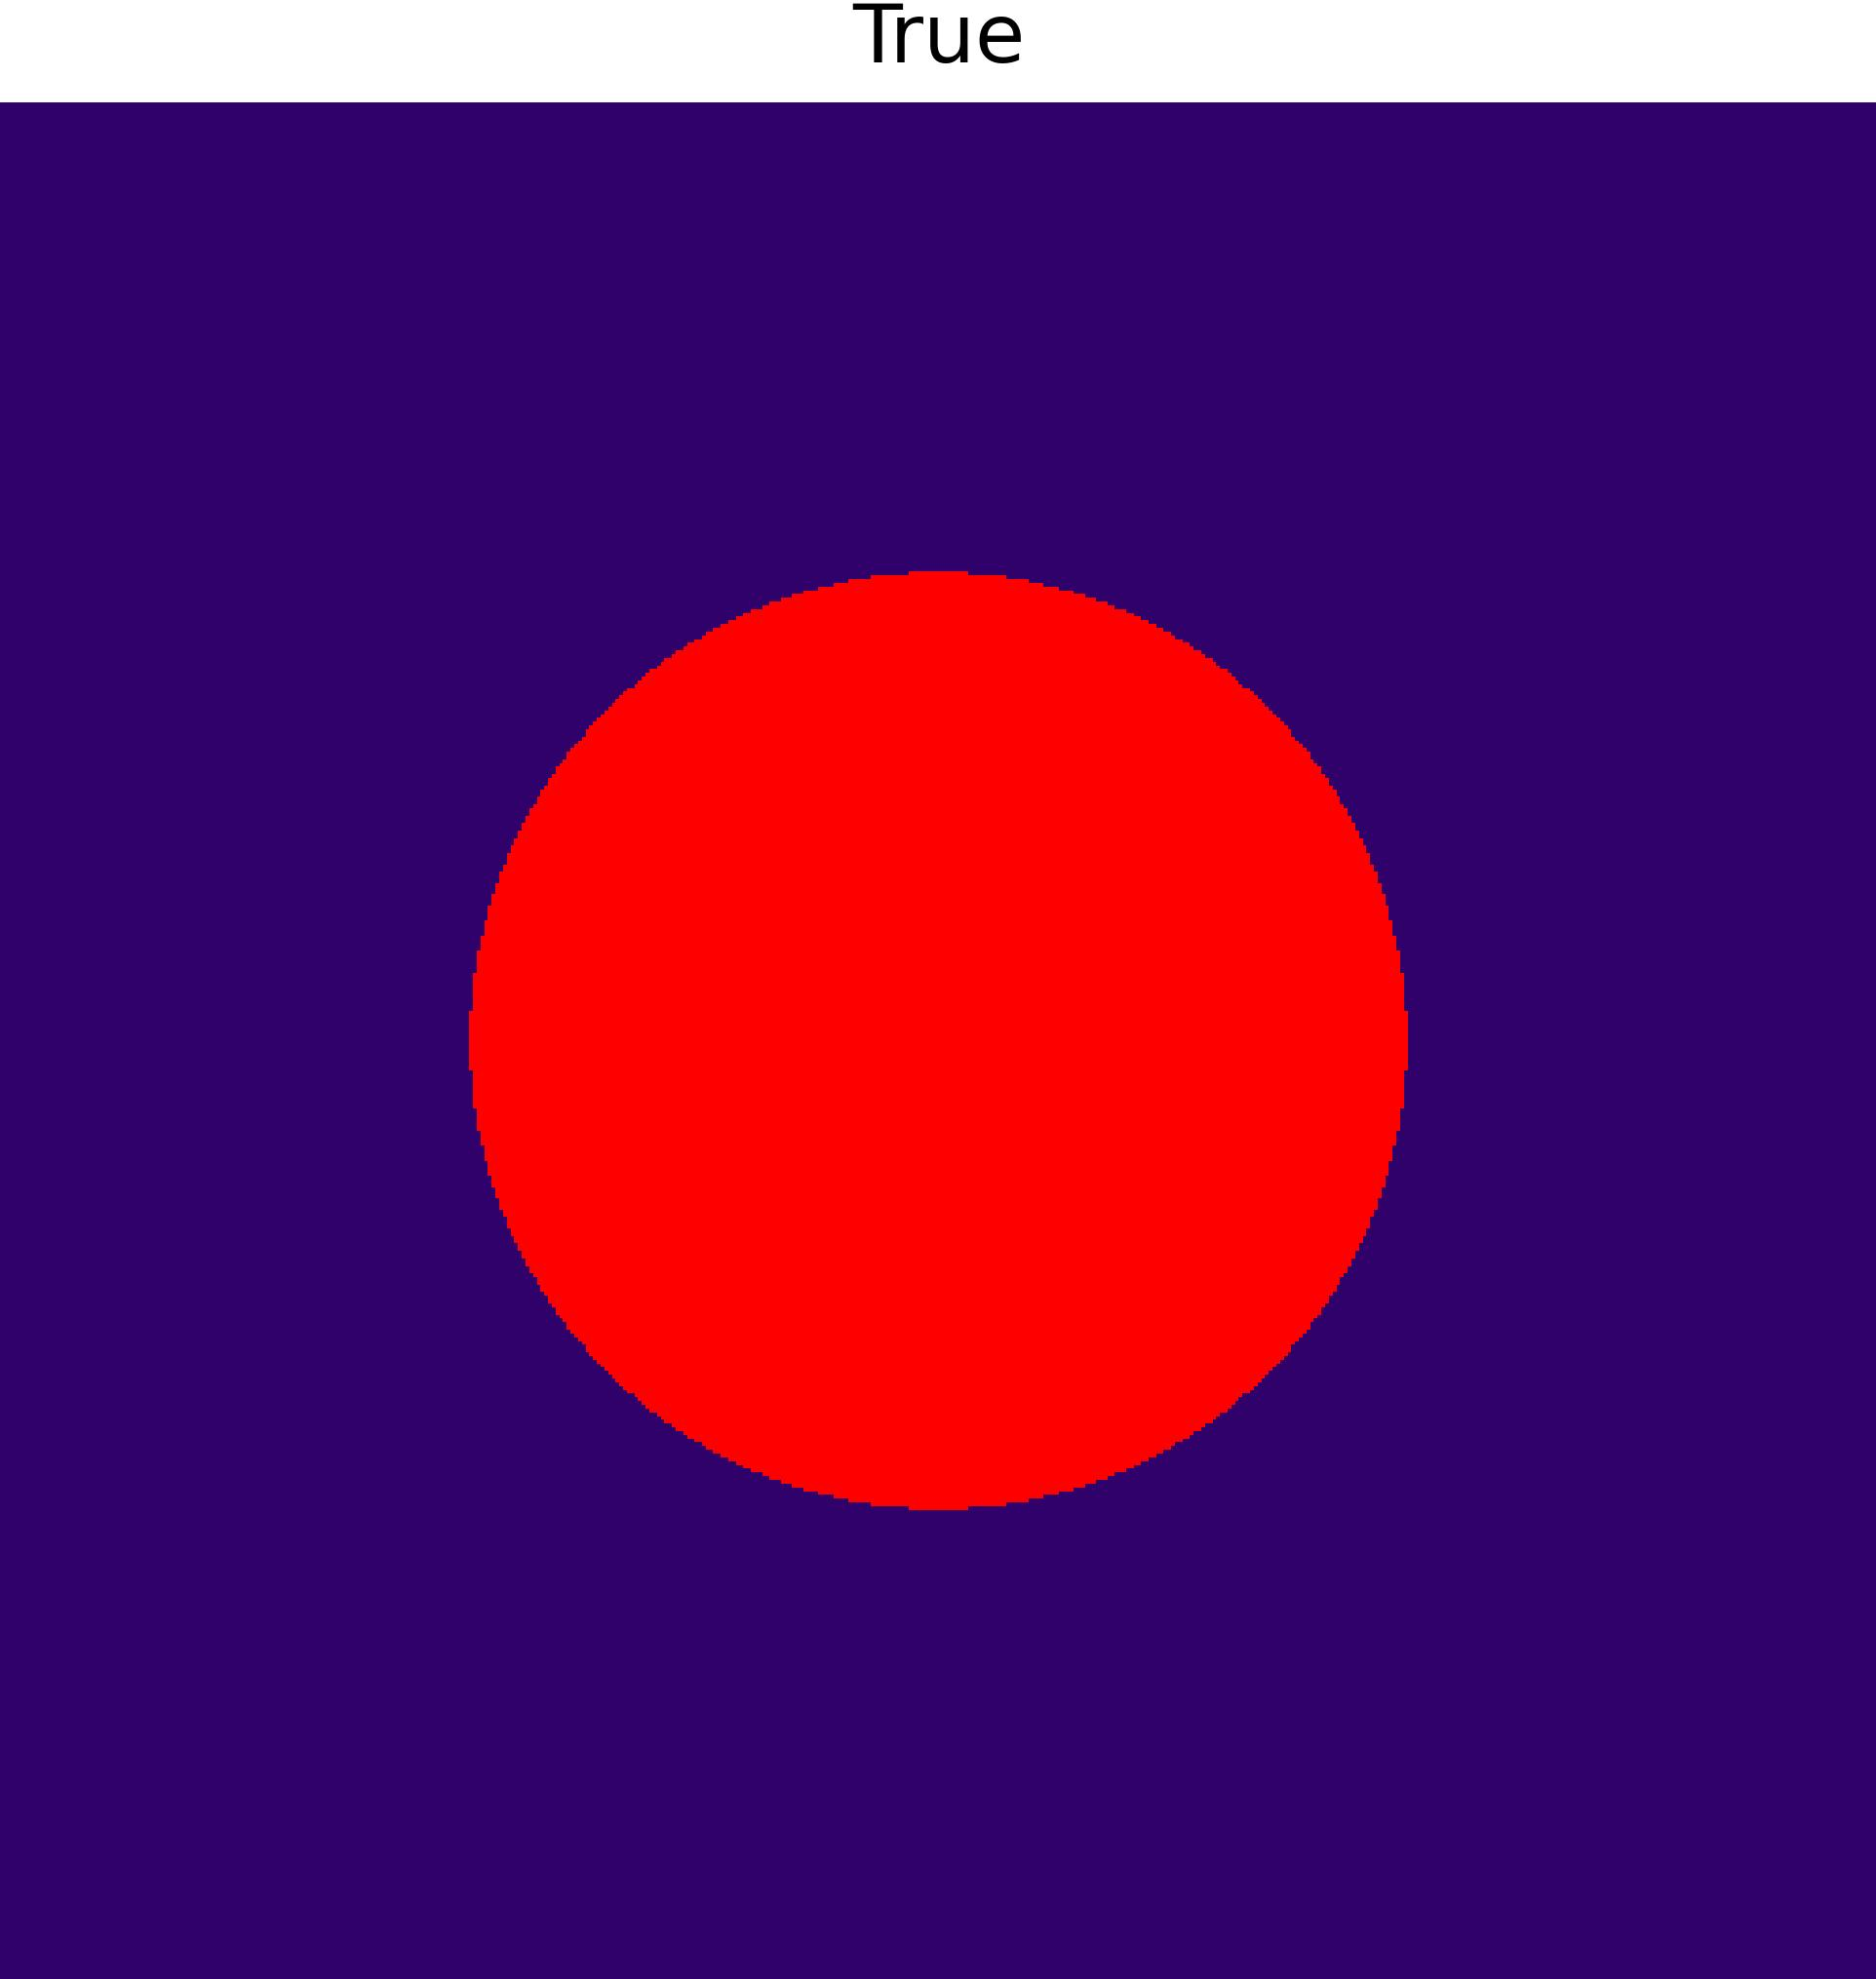
\includegraphics[height=4.5cm]{pve_true.jpg}};
		\begin{scope}[x={(img.north east)}, y={(img.south west)},visible on=<1->]
			\node[text=white, font=\scriptsize\bfseries] at (0.5,0.52) {Carotid};
			\node[text=white, font=\scriptsize\bfseries, anchor=west] at (0.8,0.52) {BG};

			\def\cx{0.50}
			\def\cy{0.50}
			\def\cr{0.25}

			% \draw[->, >=stealth, thick, white]
			% (\cx-\cr*0.25,\cy+\cr*0.65)
			% .. controls (\cx,\cy+\cr*0.90) and (\cx+\cr*0.35,\cy+\cr*0.65) ..
			% (\cx+\cr*0.15,\cy+\cr*0.30)
			% node[midway, below, text=white, font=\scriptsize] {$\omega_{c \rightarrow c}$};

			\draw[->, >=stealth, bend left=40,thick, color=white]
			(0.6,0.47) to node[above, text=white] {\small $\omega_{c\rightarrow bg}$} (0.85,0.48);

			\draw[<-, >=stealth, bend right=40,thick, color=white]
			(0.6,0.57) to node[below, text=white] {\small $\omega_{bg \rightarrow c}$} (0.85,0.56);
		\end{scope}
	\end{tikzpicture}
	% 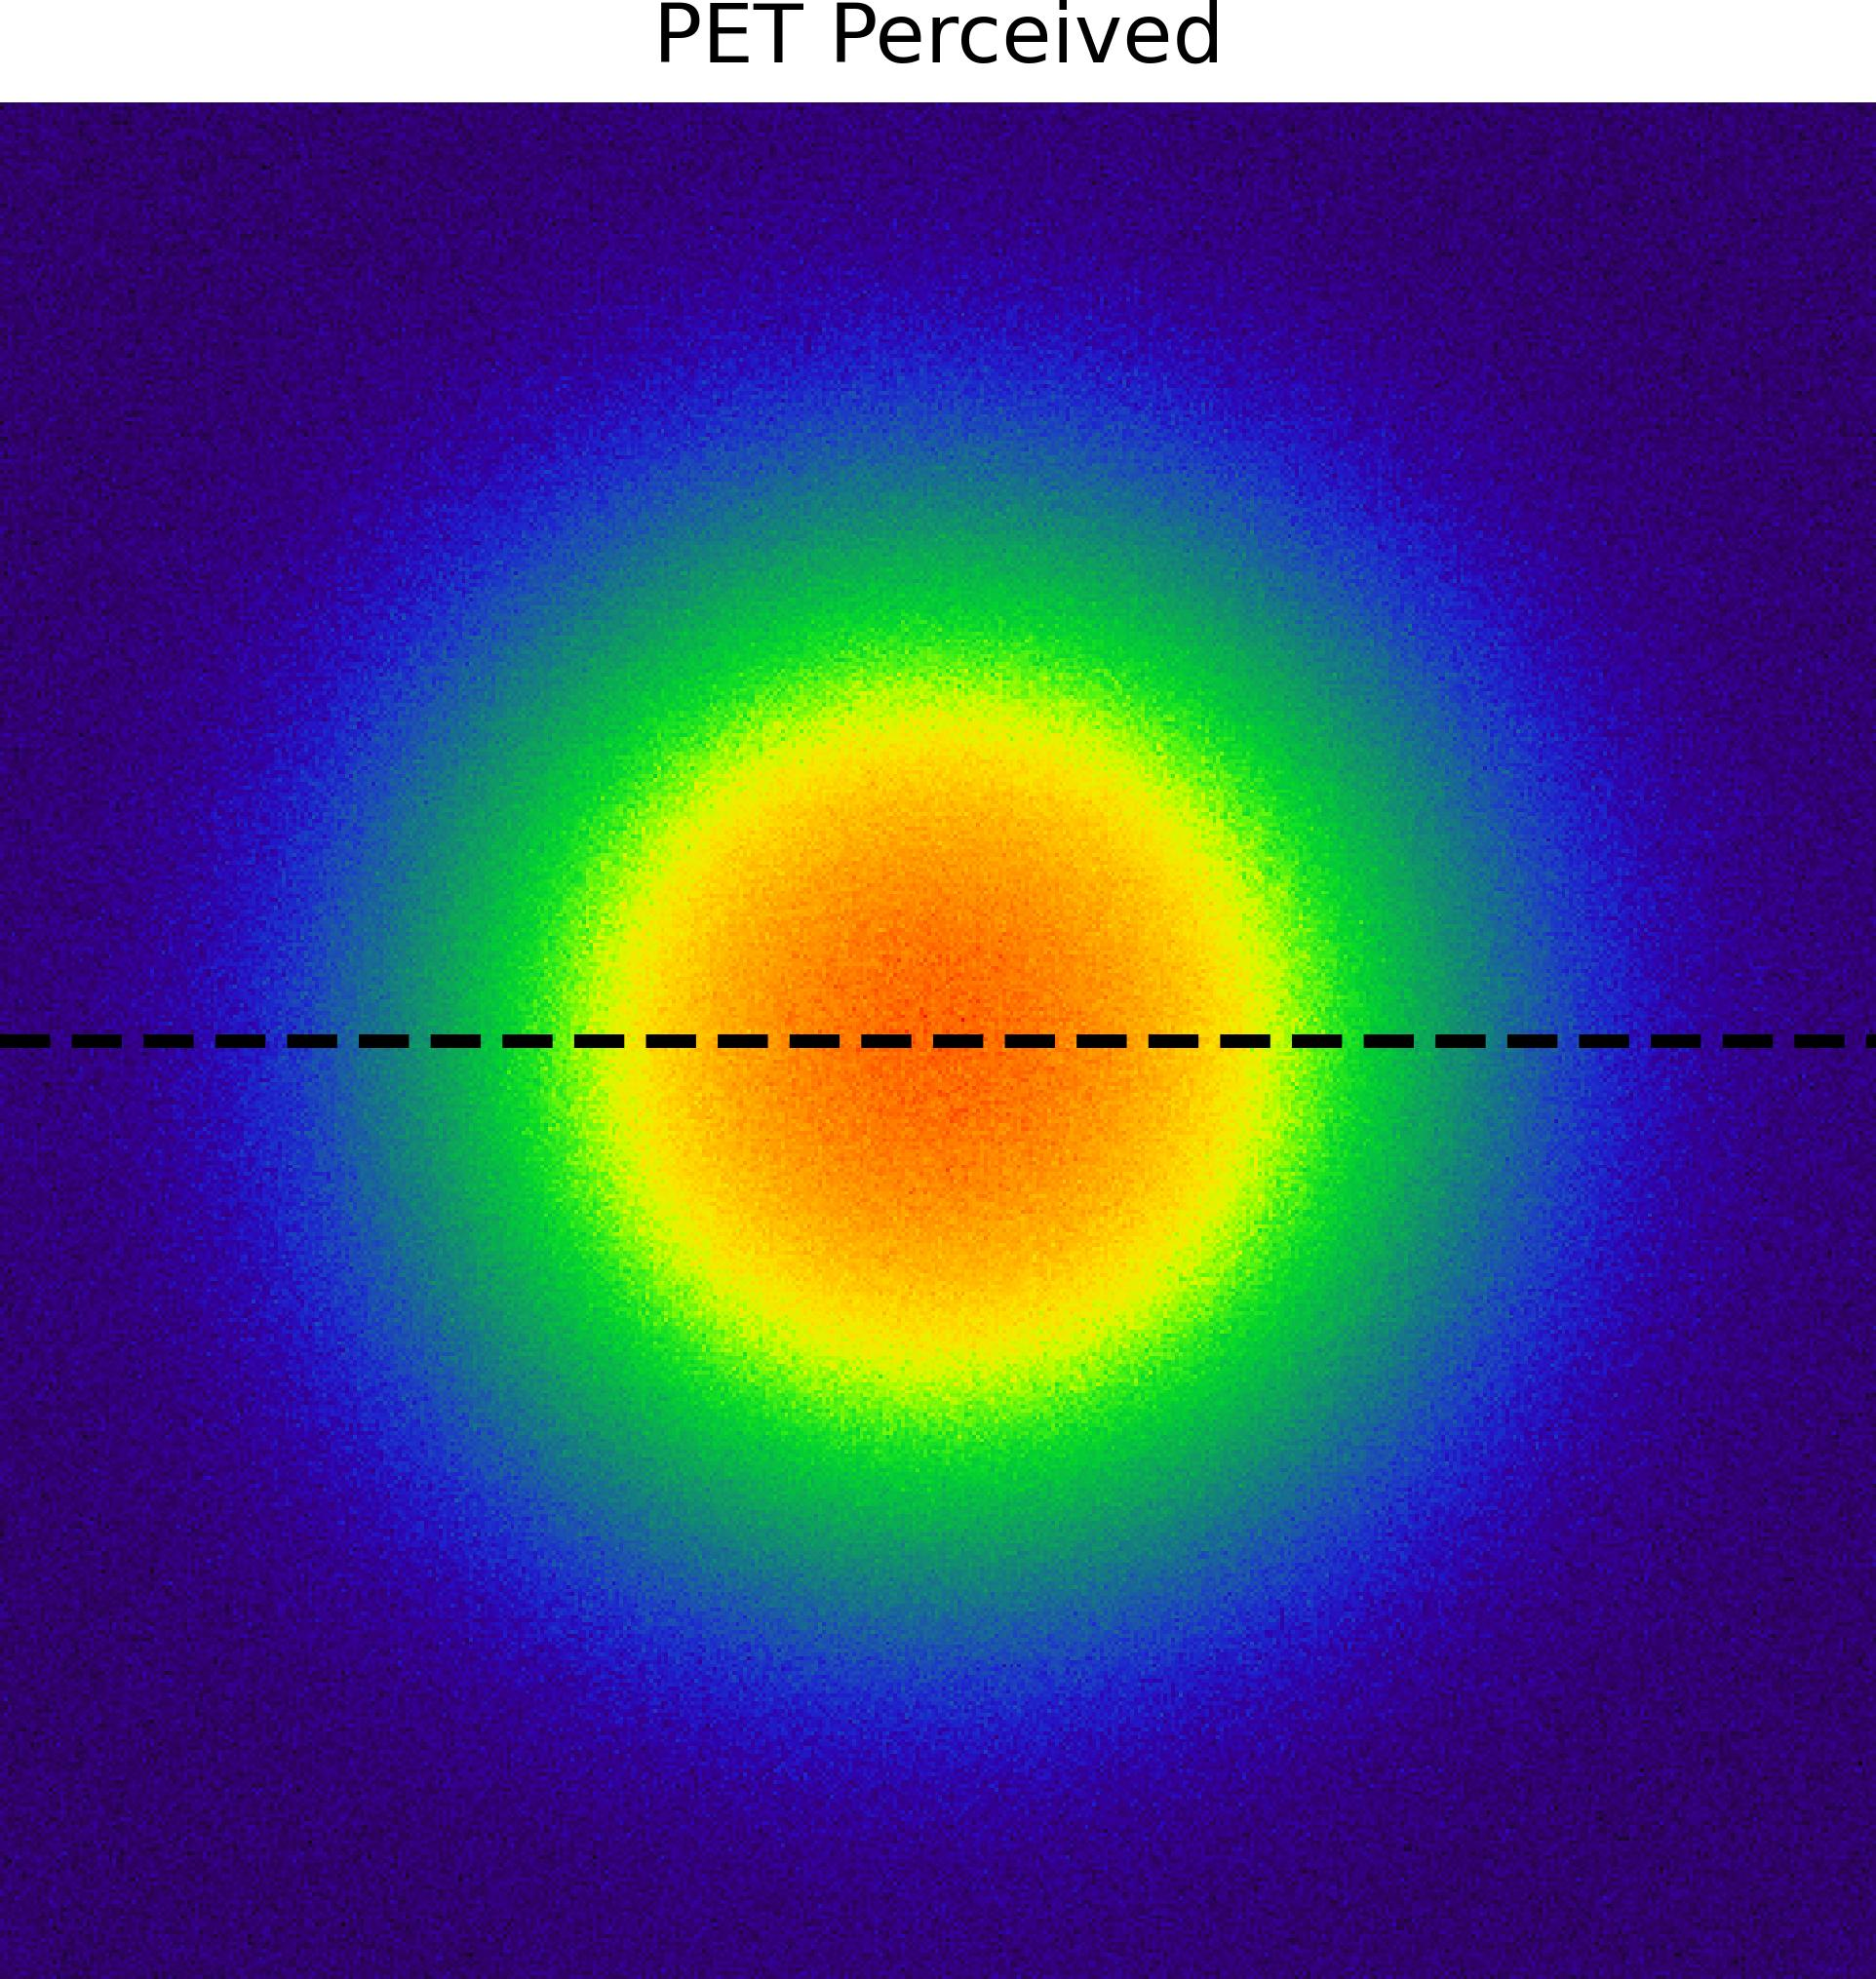
\includegraphics[height=4.5cm]{pve_perceived.jpg}
\end{frame}

\begin{frame}[t]{Geometric Transfer Matrix (GTM)}
	\centering
	\begin{center}
		% \begin{tikzpicture}
		% \end{tikzpicture}
		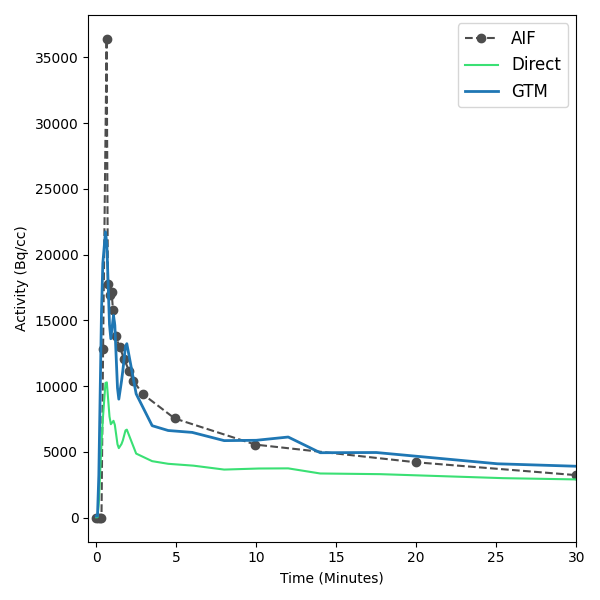
\includegraphics[height=6cm]{BADKA07504_1_bg_fg3.png}
		% \begin{tikzpicture}
		% 	\node[inner sep=0] (imgA) at (0,0)
		% 	{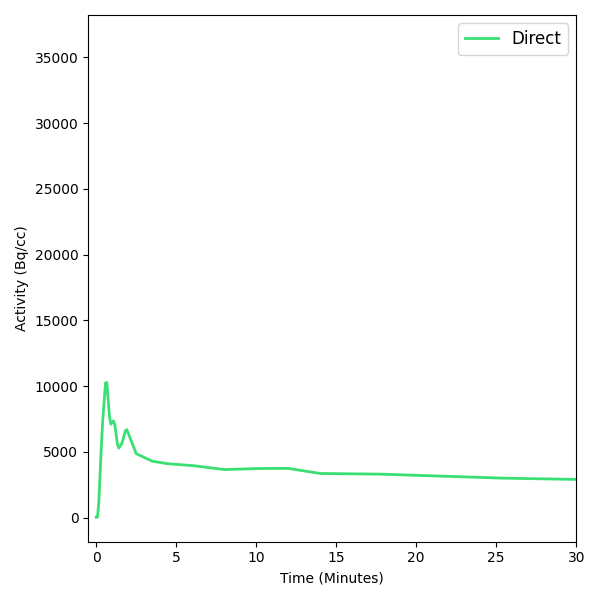
\includegraphics[height=5cm]{BADKA07504_1_bg_fg.png}};
		% 	\node[above=0cm of imgA]{$\quad$Artery};
		% 	% Second image node to the right of the first (adjust xshift if you need spacing)
		% 	\node[inner sep=0, right=0cm of imgA] (img)
		% 	{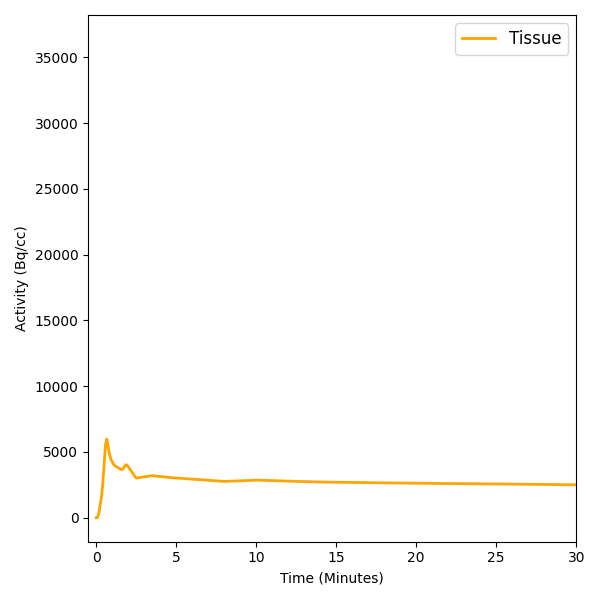
\includegraphics[height=5cm]{BADKA07504_1_bg_fg2.png}};
		% 	\node[above=0cm of img]{$\quad$Surroundings};
		%
		% 	\node[inner sep=0, right=0cm of img,visible on=<2->] (imgC)
		% 	{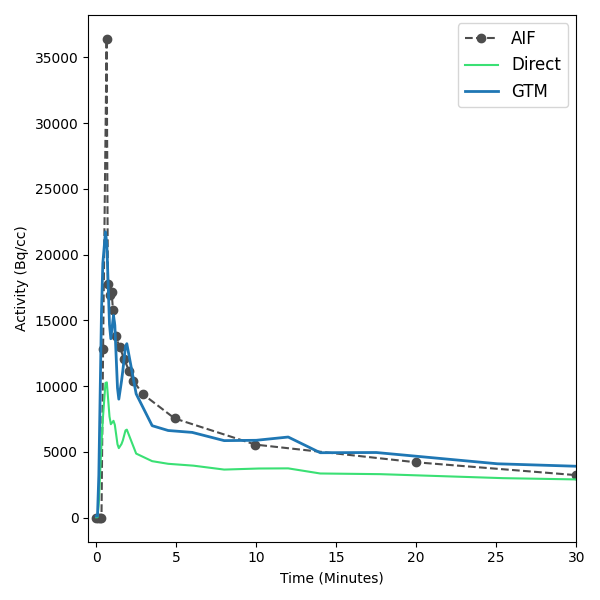
\includegraphics[height=5cm]{BADKA07504_1_bg_fg3.png}};
		% 	\node[above=0cm of imgC,visible on=<2->]{$\quad$GTM Corrected};
		%
		%
		% 	\draw[->, >=stealth, bend left=30,thick]
		% 	(1.7,2.5) to node[above] {$\omega_{out}$} (3.5,2.5);
		%
		% 	\draw[<-, >=stealth, bend right=30,thick]
		% 	(1.7,-2.5) to node[below] {\small $\omega_{in}$} (3.5,-2.5);
		% \end{tikzpicture}
		%

		\uncover<2->{\Large\textbf{Still not Accurate! The Noise is Amplified!}}
	\end{center}
\end{frame}

\begin{frame}{Modelling}
	\small
	\begin{block}{Input Function}
		\begin{itemize}
			\item PCA-based
		\end{itemize}

		\[
			T_{IF}(t) = \mu_{IF}(t) +  \textcolor{red}{\theta_1}\,v_1(t) +  \textcolor{red}{\theta_2}\,v_2(t) +  \textcolor{red}{\theta_3}\,v_3(t)
		\]
		\(\mu_{IF}(t)\): Population mean AIF (20 Random subjects from the dataset)\\
		\(v_{i}(t)\): Principal components \\
		\(\theta_{i}\): Weighting coefficients
	\end{block}
	\begin{block}{Surrounding Tissue}
		\begin{itemize}
			\item Spectral Analysis
		\end{itemize}
		\[
			T_{tissue}(t) = T_{IF} \circledast \textcolor{red}{\alpha}\,e^{-\textcolor{red}{\beta}t} (t)
		\]
	\end{block}
\end{frame}

\begin{frame}{Modelling}
	\begin{block}{Noise}
		\begin{itemize}
			\setlength\itemsep{1em}
			\item Noise in PET is multifaceted and has many different sources
			\item Noise is considered to be a time-varying Gaussian distribution
			\item It is summarized by a weighted average variance:
		\end{itemize}
		\[
			\sigma^2 = \frac{1}{N} \sum_{i=1}^{N} \omega_i\,\sigma_i^2.
		\]
		\(\omega_i\): Weighting Coefficient of frame $i$\\
		\(\sigma_i^2\): Variance of frame $i$\\
		$N$: Number of frames
		\vspace{6em}
	\end{block}
\end{frame}



\begin{frame}[t]{Bayesian GTM (BGTM)}
	\begin{block}{Summary}
		\[
			\text{IF}(t) = \mathcal{F}(\textcolor{red}{\theta_1,\theta_2,\theta_3};t),
			\quad \text{BG}(t)=\mathcal{T}(\textcolor{red}{\alpha,\beta};t),
			\quad Noise=\textcolor{red}{\sigma^2}
		\]
		\[
			\text{IF} \xleftrightarrow{\text{\quad GTM\quad}} \text{BG}
		\]
	\end{block}
	\pause
	\begin{block}{Bayesian Parameter Estimation}
		\small
		\begin{itemize}
			\item<2-> Given observed data $\mathcal{D}$, estimate $\Theta=(\textcolor{red}{\theta_1, \theta_2, \theta_3, \alpha, \beta,\mathcal{N}})$
			\item<3-> Exploration using a Markov Chain Monte-Carlo Sampler:
			      \[
				      \underbrace{p(\Theta \mid \mathcal{D})}_{\text{Posterior}} \propto \underbrace{p(\mathcal{D} \mid \Theta)}_{\text{Likelihood}} \times \underbrace{\pi(\Theta)}_{\text{Prior}}
			      \]
			\item<4-> Choose the $\Theta$ with the highest posterior:
			      \[
				      \hat{\Theta} = \arg\max_{\Theta} \left\{ p(\Theta \mid \mathcal{D}) \right\}
				      \xrightarrow{\text{Best Solution}}
				      \textcolor{OliveGreen}{\text{IF} = \mathcal{F}(\hat{\theta}_1, \hat{\theta}_2, \hat{\theta}_3)}
			      \]
		\end{itemize}
	\end{block}
\end{frame}



\section{Results}
\begin{frame}{Datasets}
	\begin{enumerate}
		\large
		\setlength\itemsep{10em}
		\item \fdg\ Dataset: 59 comatose patients
		\item \yohimbine\ Dataset: 7 healthy men
	\end{enumerate}
\end{frame}
\begin{frame}{Evaluation}
	\begin{enumerate}
		\itemsep 6em
		\large
		\item Segmentation: Visual inspection
		\item Input Function Curves: cumulative Area under the Curve (cAUC) error
		\item Regional Brain Absolute Quantification
	\end{enumerate}

\end{frame}


\begin{frame}[t]{For a Specific Subject}
	\begin{center}
		\vfill
		\begin{minipage}{0.48\textwidth}
			\centering
			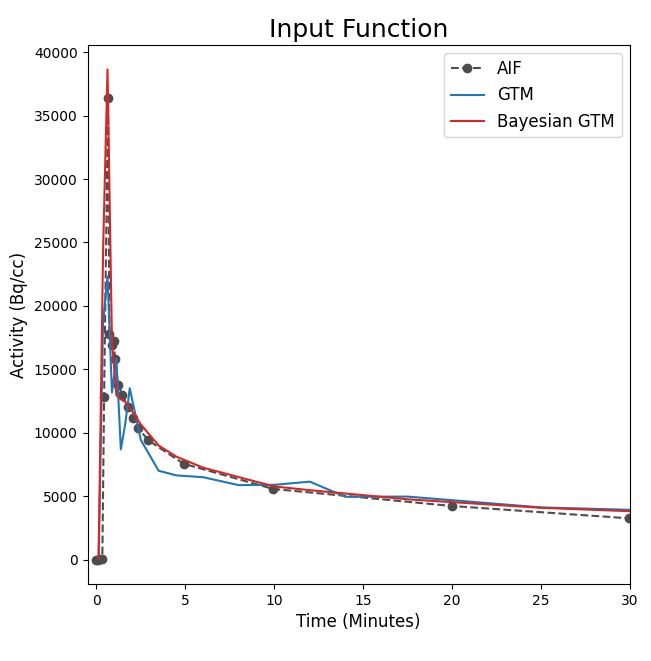
\includegraphics[width=\linewidth]{BADKA07504_1_infunc_gtm_bgtm2.png}
		\end{minipage}
		\begin{minipage}{0.48\textwidth}
			\centering
			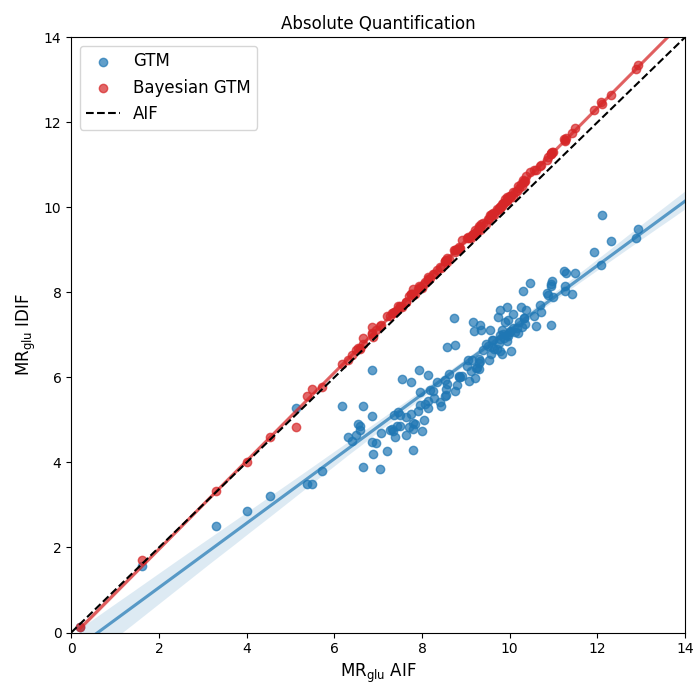
\includegraphics[width=\linewidth]{BARPH08187_1_fitk3_mrglu.png}
		\end{minipage}
		\vfill
	\end{center}
\end{frame}


\begin{frame}[t]{Overall Performance}
	Quantification error was reduced from 17\% with GTM to 10\% with Bayesian GTM
	\begin{center}
		% \includegraphics[height=0.8\textheight]{quantification_fitk3_mape_boxplot.png}
	\end{center}
\end{frame}


\begin{frame}{Conclusion}
	\begin{itemize}
		\setlength\itemsep{2em}
		\item Promising results with high clinical potential
		\item No assumptions were taken to allow for \textbf{generalizability} of the method
		\item \textbf{PET simulations} were conducted to further validate the method
		\item Independent validation is being done by Paris-Saclay with \textbf{another tracer}
		\item Method will be \textbf{submitted} in a journal by the end of the internship
	\end{itemize}

	% \vspace{1em}
	% \textbf{Personal}
	% \vspace{1em}
	%
	% \begin{itemize}
	% 	\setlength\itemsep{2em}
	%
	% 	\item Hands-on experience with conducting PET simulations
	% 	\item Enabled me to deeply understand PET kinetics and modelling
	% \end{itemize}
\end{frame}


\end{document}
